\documentclass[10pt]{article}
\usepackage[a4paper,top=2cm,bottom=2cm,left=2cm,right=2cm,marginparwidth=2cm]{geometry}
\linespread{1.5}
\usepackage[utf8]{inputenc}
\usepackage{multirow}
\usepackage{graphicx}
\usepackage{listings}
\usepackage{xcolor}
\usepackage[colorlinks=true, allcolors=black]{hyperref}
\usepackage{amsmath,amsthm,amssymb,amsfonts}
\usepackage{float}
\usepackage{listings}
\usepackage{subfigure}
\usepackage{tikz}
% \lstset{ %
%   language=R,                % the language of the code
%   basicstyle=\footnotesize,           % the size of the fonts that are used for the code
%   numbers=left,                   % where to put the line-numbers
%   numberstyle=\tiny\color[rgb]{0.4,0.2,0.2},  % the style that is used for the line-numbers
%   stepnumber=2,                   % the step between two line-numbers. If it's 1, each line 
%                                   % will be numbered
%   numbersep=12pt,                  % how far the line-numbers are from the code
%   backgroundcolor=\color{white},      % choose the background color. You must add \RequirePackage{color}
%   showspaces=false,               % show spaces adding particular underscores
%   showstringspaces=false,         % underline spaces within strings
%   showtabs=false,                 % show tabs within strings adding particular underscores
%   %frame=single,                   % adds a frame around the code
%   rulecolor=\color{black},        % if not set, the frame-color may be changed on line-breaks within not-black text (e.g. commens (green here))
%   tabsize=2,                      % sets default tabsize to 2 spaces
%   captionpos=b,                   % sets the caption-position to bottom
%   breaklines=true,                % sets automatic line breaking
%   breakatwhitespace=false,        % sets if automatic breaks should only happen at whitespace
%   title=\lstname,                   % show the filename of files included with \lstinputlisting;
%                                   % also try caption instead of title
%   keywordstyle=\color[rgb]{0.9,0.5,0.5},          % keyword style
%   commentstyle=\color[rgb]{0.4,0.3,0.9},       % comment style
%   stringstyle=\color[rgb]{0.35,0.85,0.5},         % string literal style
%   escapeinside={\%*}{*)},            % if you want to add LaTeX within your code
%   morekeywords={*,...}               % if you want to add more keywords to the set
% }

\definecolor{codegreen}{rgb}{0,0.6,0}
\definecolor{codegray}{rgb}{0.5,0.5,0.5}
\definecolor{codepurple}{rgb}{0.58,0,0.82}
\definecolor{backcolour}{rgb}{0.95,0.95,0.92}

\lstdefinestyle{mystyle}{
    backgroundcolor=\color{backcolour},   
    commentstyle=\color{codegreen},
    keywordstyle=\color{magenta},
    numberstyle=\tiny\color{codegray},
    stringstyle=\color{codepurple},
    basicstyle=\ttfamily\footnotesize,
    breakatwhitespace=false,         
    breaklines=true,                 
    captionpos=b,                    
    keepspaces=true,                 
    numbers=left,                    
    numbersep=5pt,                  
    showspaces=false,                
    showstringspaces=false,
    showtabs=false,                  
    tabsize=2
}

\lstset{style=mystyle}
\usepackage{blindtext}
\usepackage{titlesec}
\usepackage{longtable}
\graphicspath{ {./images/} }
\renewcommand{\arraystretch}{0.8}
\usepackage{amsmath} % Allows you to do equations
\usepackage{fancyhdr} % Formats the header
\setlength{\parindent}{0pt} % no paragraph indents
\setlength{\parskip}{1em} % paragraphs separated by one line
\usepackage[style=authoryear-ibid,backend=biber,maxbibnames=99,maxcitenames=2,uniquelist=false,isbn=false,url=true,hyperref=true,eprint=false,doi=true,giveninits=true,uniquename=init]{biblatex} % Allows you to do citations - does Harvard style and compatible with Zotero
%\usepackage[style=authoryear, citestyle=authoryear, backend=biber]{biblatex}
\usepackage[colorlinks,citecolor=blue,urlcolor=blue,bookmarks=false,hypertexnames=true]{hyperref} 

\defbibenvironment{bibliography}
  {\list
     {\printtext[labelalphawidth]{%
        \printfield{labelprefix}%
        \printfield{labelalpha}%
        \printfield{extraalpha}}}
     {\setlength{\labelwidth}{\labelalphawidth}%
      \setlength{\leftmargin}{\labelwidth}%
      \setlength{\labelsep}{\biblabelsep}%
      \addtolength{\leftmargin}{\labelsep}%
      \setlength{\itemsep}{\bibitemsep}%
      \setlength{\parsep}{\bibparsep}}%
      \renewcommand*{\makelabel}[1]{##1\hss}}
  {\endlist}
  {\item}
\addbibresource{name.bib}

\renewcommand{\headrulewidth}{0pt}
\geometry{letterpaper, portrait, margin=1in}
\setlength{\headheight}{14.49998pt}

\newcommand\titleofdoc{ECON 723 Econometrics II} %%%%% Put your document title in this argument
\newcommand\GroupName{name} %%%%% Put your group name here. If you are the only member of the group, just put your name

\begin{document}
\begin{titlepage}
   \begin{center}
        \vspace*{3cm} % Adjust spacings to ensure the title page is generally filled with text

        \Large{\titleofdoc} 

        \vspace{0.5cm}
        \LARGE{ECON 723 Group Project 1}
            
        \vspace{2 cm}
        \Large{}
            
        \vspace{2 cm}
        \Large{\GroupName}
       
        \vspace{0.25cm}
        \large{id}
       
        \vspace{1 cm}
        \Large{22 Jun 2023}
        
        \vspace{0.25 cm}
        \Large{ }
       

       \vfill
    \end{center}
\end{titlepage}

\newpage

\setcounter{page}{1}
\pagestyle{fancy}
\fancyhf{}
\rhead{\thepage}
\lhead{\GroupName; \titleofdoc}


\def\
% Add subject and keywords below
\hypersetup{
     %pdfsubject={The Subject},
     %pdfkeywords={Some Keywords},
     pdfauthor={Kim Jin},
     pdftitle={ECON 721 project}
     }




\section*{Abstract}



\newpage
\tableofcontents

\newpage
\pagenumbering{arabic}

\section{Overview}



\section{Literature Review}



\section{Data Acquisition and Management}

\subsection{Data Sources}
Our dataset comprises the monthly yields for 1, 2, 5, and 10-year periods for both New Zealand (NZ) and the United States (US). Additionally, it includes the exchange rates and 90 day bank bill yields from both countries.



\subsection{Data Enrichment}

Being a time series dataset, our primary focus is to ascertain the presence of trends, seasonality, autocorrelation, and its stationarity. For this, we decomposed the time series data into its constituent elements: the seasonal, trend, and random (or irregular) components.

To achieve this, we utilized the decompose model. An analysis of the resultant table suggests an absence of a distinct trend. However, the data exhibits clear seasonality while appearing somewhat random.

\[Y_{t}=Trend_{t}+Seasonal_{t}+Random_{t}\]

From the table, we can see that there is not a clear trend and clearly the data is seasonal, and it looks random.

\begin{figure}[H]
    \centering
    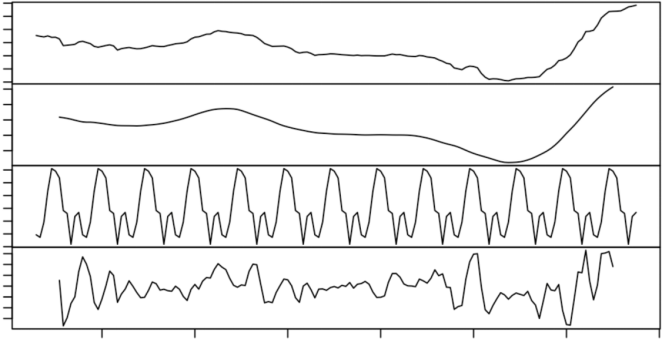
\includegraphics[width=0.8\textwidth]{work/picture/Decomposition.png}
  \vspace{20pt}\caption{\hyperref[Decomposition1]{Decomposition of additive time series}}
  %  \label{Decomposition1}
    \begin{picture}(0,0)
        \put(0.37\textwidth,0.097\textwidth){\makebox(0,0)[lt]{\small{{2024}}}}
        \put(0.26\textwidth,0.097\textwidth){\makebox(0,0)[lt]{\small{{2022}}}}
        \put(0.15\textwidth,0.097\textwidth){\makebox(0,0)[lt]{\small{{2020}}}}
        \put(0.04\textwidth,0.097\textwidth){\makebox(0,0)[lt]{\small{{2018}}}}
        \put(-0.07\textwidth,0.097\textwidth){\makebox(0,0)[lt]{\small{{2016}}}}
        \put(-0.18\textwidth,0.097\textwidth){\makebox(0,0)[lt]{\small{{2014}}}}
        \put(-0.29\textwidth,0.097\textwidth){\makebox(0,0)[lt]{\small{{2012}}}}

        \put(-0.43\textwidth,0.14\textwidth){\makebox(0,0)[lt]{\rotatebox{90}{\small{-0.3}}}}
        \put(-0.43\textwidth,0.19\textwidth){\makebox(0,0)[lt]{\rotatebox{90}{\small{0.1}}}}
        \put(-0.43\textwidth,0.23\textwidth){\makebox(0,0)[lt]{\rotatebox{90}{\small{-0.06}}}}
        \put(-0.43\textwidth,0.286\textwidth){\makebox(0,0)[lt]{\rotatebox{90}{\small{0.02}}}}
        \put(-0.43\textwidth,0.334\textwidth){\makebox(0,0)[lt]{\rotatebox{90}{\small{1}}}}
        \put(-0.43\textwidth,0.37\textwidth){\makebox(0,0)[lt]{\rotatebox{90}{\small{3}}}}
        \put(-0.43\textwidth,0.415\textwidth){\makebox(0,0)[lt]{\rotatebox{90}{\small{50}}}}
        \put(-0.43\textwidth,0.45\textwidth){\makebox(0,0)[lt]{\rotatebox{90}{\small{2}}}}
        \put(-0.43\textwidth,0.48\textwidth){\makebox(0,0)[lt]{\rotatebox{90}{\small{4}}}}
        \put(-0.43\textwidth,0.51\textwidth){\makebox(0,0)[lt]{\rotatebox{90}{\small{6}}}}

        \put(-0.02\textwidth,0.07\textwidth){\makebox(0,0)[lt]{\textbf{Time}}}
        \put(-0.47\textwidth,0.47\textwidth){\makebox(0,0)[lt]{\rotatebox{90}{\textbf{random seasonal trend observed}}}}

    \end{picture}
\end{figure}


It's worth noting that a non-stationary time series will always contain the a random, volatile component. This component encapsulates minor fluctuations around the overarching trend, cycle, and seasonal elements. While unpredictable, this can typically be modeled as random observations deriving from a certain distribution, often represented as \(N(0,\sigma^2)\).
\subsubsection{ACF test}

\tikzset{global scale/.style={
    scale=#1,
    every node/.append style={scale=#1}
  }
}
\begin{figure}[H]
    \centering
        \begin{tikzpicture}[global scale = 1]
            \node[anchor=south west,inner sep=0] at (0,0) {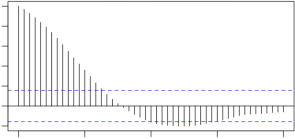
\includegraphics[width=0.3\textwidth]{work/picture/Series1.png}};
    \node at(0.35,-0.15){\small 0};
    \node at(1.49,-0.15){\small 1};     
    \node at(2.63,-0.15){\small 2};
    \node at(3.77,-0.15){\small 3};   
    \node at(4.92,-0.15){\small 4};
    \node at(2.63,-0.8){\small Lag};
    \node at(2.63,2.8){ \hyperref[Series1]{\textbf{Series swap.ts}}};

    \node at(-0.2,0.2)[rotate=90]{\small -0.2};        
    \node at(-0.2,0.9)[rotate=90]{\small 0.2};  
    \node at(-0.2,1.6)[rotate=90]{\small 0.6};  
    \node at(-0.2,2.3)[rotate=90]{\small 1.0};  
    \node at(-1,1.2)[rotate=90]{\small ACF};        

    
            \node[anchor=south west,inner sep=0] at (7,0) {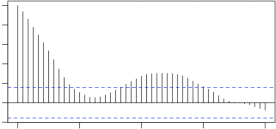
\includegraphics[width=0.3\textwidth]{work/picture/Series2.png}};
            \node at(9.5,2.8){\hyperref[Series2]{\textbf{Series (swap.ts-mean(swap.ts))$^2$}}};
     \node at(7+0.35,-0.15){\small 0};
    \node at(7+1.49,-0.15){\small 1};     
    \node at(7+2.63,-0.15){\small 2};
    \node at(7+3.77,-0.15){\small 3};   
    \node at(7+4.92,-0.15){\small 4};
    \node at(7+2.63,-0.8){\small Lag};

    \node at(7+-0.2,0.2)[rotate=90]{\small -0.2};        
    \node at(7+-0.2,0.9)[rotate=90]{\small 0.2};  
    \node at(7+-0.2,1.6)[rotate=90]{\small 0.6};  
    \node at(7+-0.2,2.3)[rotate=90]{\small 1.0};  
    \node at(7+-1,1.2)[rotate=90]{\small ACF};   
        \end{tikzpicture}
    \caption{}
 %   \label{Series1}
\end{figure}

The Autocorrelation Function (ACF) points to a robust autocorrelation at lag(16) in the swap rate, hinting at seasonality. It is observed that as time progresses, the positive correlation tends to wane until it turns negative. However, this correlation also diminishes with increasing lag. Our primary focus is on data points outside the blue region, given their high statistical significance. An analysis of heteroscedasticity corroborates these findings.

\begin{lstlisting}[language = R]
        Augmented Dickey-Fuller Test
    
data: swap.ts
Dickey-Fuller  =-1.0953, Lag order  =5, p -value  =0.9203  
alternative hypothesis: stationary    

\end{lstlisting}

\subsubsection{The ADF test:}

For a time series to be classified as stationary, it must be devoid of trends or seasonal impacts. If the procured p-value surpasses the significance level of 0.05 and the ADF statistic is greater than any of the established critical values, we have no compelling reason to reject the null hypothesis. As such, our conclusion is that the time series is non-stationary.

Furthermore, a similar analysis was conducted for the two-year period swap rate. The findings paralleled the observations made previously.

\begin{lstlisting}[language = R]
        Augmented Dickey-Fuller Test
        
data: swap.ts1
Dickey-Fuller  = -0.96763, Lag order  = 5, p-value  = 0.9405 
alternative hypothesis: stationary  

\end{lstlisting}


\begin{figure}[H]
    \centering
        \begin{tikzpicture}[global scale = 1]
            \node[anchor=south west,inner sep=0] at (0,0) {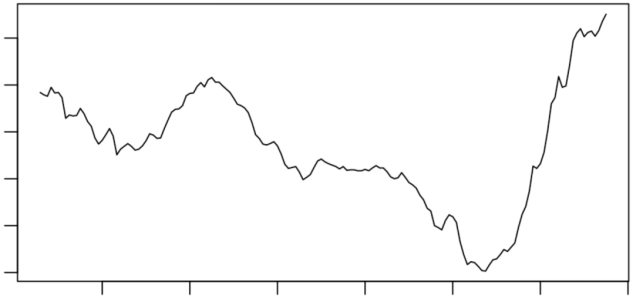
\includegraphics[width=0.8\textwidth]{work/picture/Swap.png}};
    \node at(13.3,-0.3){\small 2024};
    \node at(11.45,-0.3){\small 2022};     
    \node at(9.6,-0.3){\small 2020}; 
    \node at(7.75,-0.3){\small 2018}; 
    \node at(5.9,-0.3){\small 2016}; 
    \node at(4.05,-0.3){\small 2014}; 
    \node at(2.2,-0.3){\small 2012};    
    \node at(6.7,-1){\small month};   


    

    \node at(-0.3,0.5)[rotate=90]{\small 0};    
    \node at(-0.3,1.5)[rotate=90]{\small 1};   
    \node at(-0.3,2.5)[rotate=90]{\small 2};    
    \node at(-0.3,3.5)[rotate=90]{\small 3};   
    \node at(-0.3,4.5)[rotate=90]{\small 4};    
    \node at(-0.3,5.5)[rotate=90]{\small 5};   
    \node at(-1,3)[rotate=90]{\small Swap Rate in Percent};   
    
        \end{tikzpicture}
    \caption{\hyperref[Swap]{Swap Rate for 2 Year Period}}
 %   \label{Swap}
\end{figure}


\begin{figure}[H]
    \centering
        \begin{tikzpicture}[global scale = 1]
            \node[anchor=south west,inner sep=0] at (0,0) {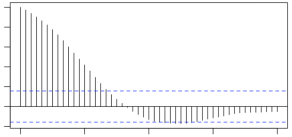
\includegraphics[width=0.3\textwidth]{work/picture/Series2_1.png}};
    \node at(0.35,-0.15){\small 0};
    \node at(1.49,-0.15){\small 1};     
    \node at(2.63,-0.15){\small 2};
    \node at(3.77,-0.15){\small 3};   
    \node at(4.92,-0.15){\small 4};
    \node at(2.63,-0.8){\small Lag};
    \node at(2.63,2.8){ \hyperref[Series21]{\textbf{Series swap.ts1}}};

    \node at(-0.2,0.2)[rotate=90]{\small -0.2};        
    \node at(-0.2,0.9)[rotate=90]{\small 0.2};  
    \node at(-0.2,1.6)[rotate=90]{\small 0.6};  
    \node at(-0.2,2.3)[rotate=90]{\small 1.0};  
    \node at(-1,1.2)[rotate=90]{\small ACF};        

    
            \node[anchor=south west,inner sep=0] at (7,0) {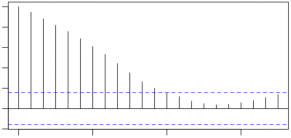
\includegraphics[width=0.3\textwidth]{work/picture/Series2_2.png}};
            \node at(9.5,2.8){ \hyperref[Series22]{\textbf{Series (swap.ts1-mean(swap.ts1))$^2$}}};

    \node at(7+0.4,-0.15){\small 0.0};     
    \node at(7+1.7,-0.15){\small 0.5};
    \node at(7+3,-0.15){\small 1.0};   
    \node at(7+4.3,-0.15){\small 1.5};
    \node at(7+2.63,-0.8){\small Lag};

    \node at(7+-0.2,0.2)[rotate=90]{\small -0.0};        
    \node at(7+-0.2,0.9)[rotate=90]{\small 0.2};  
    \node at(7+-0.2,1.6)[rotate=90]{\small 0.6};  
    \node at(7+-0.2,2.3)[rotate=90]{\small 1.0};  
    \node at(7+-1,1.2)[rotate=90]{\small ACF};   
        \end{tikzpicture}
    \caption{}
   % \label{Series2}
\end{figure}

\begin{figure}[H]
    \centering
    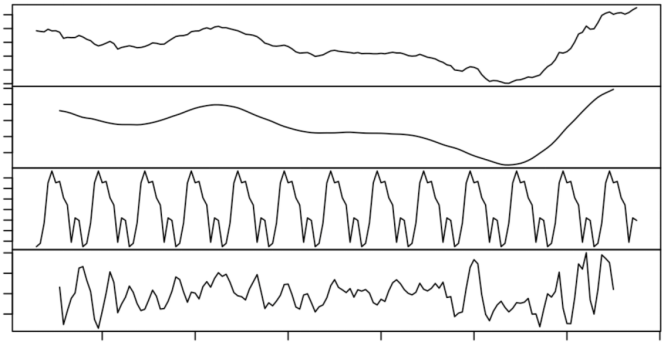
\includegraphics[width=0.8\textwidth]{work/picture/Decomposition2.png}
  \vspace{20pt}\caption{\hyperref[Decomposition2]{Decomposition of additive time series}}
 %   \label{Decomposition}

    \begin{picture}(0,0)
        \put(0.37\textwidth,0.097\textwidth){\makebox(0,0)[lt]{\small{{2024}}}}
        \put(0.26\textwidth,0.097\textwidth){\makebox(0,0)[lt]{\small{{2022}}}}
        \put(0.15\textwidth,0.097\textwidth){\makebox(0,0)[lt]{\small{{2020}}}}
        \put(0.04\textwidth,0.097\textwidth){\makebox(0,0)[lt]{\small{{2018}}}}
        \put(-0.075\textwidth,0.097\textwidth){\makebox(0,0)[lt]{\small{{2016}}}}
        \put(-0.19\textwidth,0.097\textwidth){\makebox(0,0)[lt]{\small{{2014}}}}
        \put(-0.3\textwidth,0.097\textwidth){\makebox(0,0)[lt]{\small{{2012}}}}

        \put(-0.43\textwidth,0.16\textwidth){\makebox(0,0)[lt]{\rotatebox{90}{\small{-0.2}}}}
        \put(-0.43\textwidth,0.205\textwidth){\makebox(0,0)[lt]{\rotatebox{90}{\small{0.2}}}}
        \put(-0.43\textwidth,0.25\textwidth){\makebox(0,0)[lt]{\rotatebox{90}{\small{-0.06}}}}
        \put(-0.43\textwidth,0.306\textwidth){\makebox(0,0)[lt]{\rotatebox{90}{\small{0.02}}}}
        \put(-0.43\textwidth,0.348\textwidth){\makebox(0,0)[lt]{\rotatebox{90}{\small{1}}}}
        \put(-0.43\textwidth,0.383\textwidth){\makebox(0,0)[lt]{\rotatebox{90}{\small{3}}}}
        \put(-0.43\textwidth,0.425\textwidth){\makebox(0,0)[lt]{\rotatebox{90}{\small{50}}}}
        \put(-0.43\textwidth,0.46\textwidth){\makebox(0,0)[lt]{\rotatebox{90}{\small{2}}}}
        \put(-0.43\textwidth,0.49\textwidth){\makebox(0,0)[lt]{\rotatebox{90}{\small{4}}}}

        \put(-0.02\textwidth,0.07\textwidth){\makebox(0,0)[lt]{\textbf{Time}}}
        \put(-0.47\textwidth,0.47\textwidth){\makebox(0,0)[lt]{\rotatebox{90}{\textbf{Random Seasonal Trend Observed}}}}

    \end{picture}
\end{figure}



\subsection{Predicting Yield Rates Using Swap Rates}


\begin{figure}[H]
    \centering
        \begin{tikzpicture}[global scale = 1]
            \node[anchor=south west,inner sep=0] at (0,0) {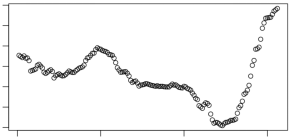
\includegraphics[width=0.3\textwidth]{work/picture/Swap2_1.png}};
    \node at(0.35,-0.15){\small 0};
    \node at(1.74,-0.15){\small 50};     
    \node at(3.2,-0.15){\small 100};
    \node at(4.65,-0.15){\small 150};   
    \node at(2.7,-0.8){\small month};
    \node at(2.63,2.8){ \hyperref[Swap21]{\textbf{Swap Rate for 1 Year Period}}};

    \node at(-0.2,0.2)[rotate=90]{\small 0};    
       \node at(-0.2,0.55)[rotate=90]{\small 1}; 
    \node at(-0.2,0.9)[rotate=90]{\small 2};  
    \node at(-0.2,1.25)[rotate=90]{\small 3};
    \node at(-0.2,1.6)[rotate=90]{\small 4};  
    \node at(-0.2,1.95)[rotate=90]{\small 5};
    \node at(-0.2,2.3)[rotate=90]{\small 6};  
    \node at(-1,1.2)[rotate=90]{\small Swap Rate in Percent};        

    
            \node[anchor=south west,inner sep=0] at (7,0) {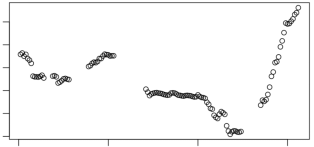
\includegraphics[width=0.3\textwidth]{work/picture/Yields.png}};
            \node at(9.5,2.8){ \hyperref[Yields2]{\textbf{Yields Rate for 1 Year Period}}};

    \node at(7+0.35,-0.15){\small 0};
    \node at(7+1.74,-0.15){\small 50};     
    \node at(7+3.2,-0.15){\small 100};
    \node at(7+4.65,-0.15){\small 150};   
    \node at(7+2.7,-0.8){\small Month};


     \node at(7-0.2,0.2)[rotate=90]{\small 0};    
       \node at(7+-0.2,0.55)[rotate=90]{\small 1}; 
    \node at(7+-0.2,0.9)[rotate=90]{\small 2};  
    \node at(7+-0.2,1.25)[rotate=90]{\small 3};
    \node at(7+-0.2,1.6)[rotate=90]{\small 4};  
    \node at(7+-0.2,1.95)[rotate=90]{\small 5};

     \node at(6,1.2)[rotate=90]{\small Yields Rate in Percent};   
        \end{tikzpicture}
    \caption{}
  %  \label{Series2}
\end{figure}

\subsubsection{Correlation Between Swap and Yield Rates}

We initiated our analysis by graphing the trends between the swap and yield rates. A visual inspection suggests a potential correlation. This observation led us to employ regression using data from both the yield and swap rates. The following regression model was proposed:
\[Yield\_1year_{i}=c+\beta \cdot Swap\_rate\_1year_{i}+\epsilon_{i}\]

\begin{lstlisting}
Call:
 lm(formula  =  data$bond_closing_yields_1year ~data$Swap_rates_1year)

Residuals:
     Min      1 Q    Median       3Q      Max  
-0.34417  -0.06211 -0.02351  0.05513  0.42781


Coefficients:
                        Estimate Std. Error t value Pr(>|t|)
(Intercept)            -0.047444   0.027415  -1.731   0.0863 .
data$Swap_rates_1year   0.936676   0.009457  99.050   <2 e-16 *** 
---
Signif. codes: 0 '* * *', 0.001 '* *', 0.01 '*', 0.05 '.', 0.1  '' 1
Residual standard error: 0.1328 on 113 degrees of freedom 
  (41 observations deleted due to missingness)
Multiple R-squared: 0.9886,  Adjusted R-squared: 0.9885
F-statistic: 9811 on 1 and 113 DF, p-value: < 2.2e-16    
\end{lstlisting}

\subsubsection{Omitted Variable Bias}
Though the model appeared to be significant, closer scrutiny of the one-year yield rate revealed gaps in the data for specific years. Relying solely on simple linear regression for prediction in such cases can lead to omitted variable bias. This necessitates the exploration of alternative, more reliable methods. The issue of missing data persisted when considering the two-year period.


\begin{lstlisting}
Call:
lm(formula  =  data$bond_closing_yields_2year ~ data$Swap_rates_2year)

Residuals:
      Min        1Q    Median       3Q      Max  
 -0.42686  -0.10933  -0.01985  0.06238  0.54959
 
Coefficients:
                        Estimate Std. Error t value Pr(>|t|)
(Intercept)             -0.13826    0.03648   -3.79 0.000229 *** 
data$Swap_rates_2year    0.96271    0.01245   77.33 <2 e-16 *** 

Residual standard error: 0.1628 on 130 degrees of freedom
(24 observations deleted due to missingness)
Multiple R-squared: 0.9787,  Adjusted R-squared: 0.9786
F-statistic: 5980 on 1 and 130 DF, p-value: < 2.2e-16    
\end{lstlisting}





\begin{figure}[H]
    \centering
        \begin{tikzpicture}[global scale = 1]
            \node[anchor=south west,inner sep=0] at (0,0) {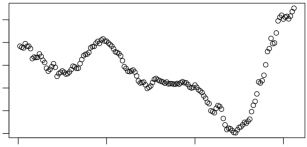
\includegraphics[width=0.3\textwidth]{work/picture/Swap3_1.png}};
    \node at(0.35,-0.15){\small 0};
    \node at(1.74,-0.15){\small 50};     
    \node at(3.2,-0.15){\small 100};
    \node at(4.65,-0.15){\small 150};   
    \node at(2.7,-0.8){\small month};
    \node at(2.63,2.8){ \hyperref[Swap31]{\textbf{Swap Rate for 2 Year Period}}};

    \node at(-0.2,0.2)[rotate=90]{\small 0};    
       \node at(-0.2,0.6)[rotate=90]{\small 1}; 
    \node at(-0.2,0.95)[rotate=90]{\small 2};  
    \node at(-0.2,1.35)[rotate=90]{\small 3};
    \node at(-0.2,1.72)[rotate=90]{\small 4};  
    \node at(-0.2,2.1)[rotate=90]{\small 5};
    \node at(-1,1.2)[rotate=90]{\small Swap Rate in Percent};        

    
            \node[anchor=south west,inner sep=0] at (7,0) {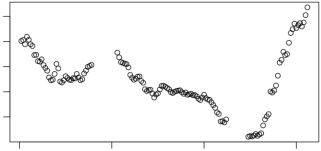
\includegraphics[width=0.3\textwidth]{work/picture/Yield3_2.png}};
            \node at(9.5,2.8){ \hyperref[Yields32]{\textbf{Yields Rate for 2 Year Period}}};

    \node at(7+0.35,-0.15){\small 0};
    \node at(7+1.74,-0.15){\small 50};     
    \node at(7+3.2,-0.15){\small 100};
    \node at(7+4.65,-0.15){\small 150};   
    \node at(7+2.7,-0.8){\small month};


     \node at(7-0.2,0.2+0.35)[rotate=90]{\small 1};    
       \node at(7+-0.2,0.55+0.36)[rotate=90]{\small 2}; 
    \node at(7+-0.2,0.9+0.41)[rotate=90]{\small 3};  
    \node at(7+-0.2,1.25+0.43)[rotate=90]{\small 4};
    \node at(7+-0.2,1.6+0.49)[rotate=90]{\small 5};  


     \node at(6,1.2)[rotate=90]{\small Yields Rate in Percent};   
        \end{tikzpicture}
    \caption{}
    %\label{Series2}
\end{figure}


\subsection{Machine Learning – The Random Forest Model}
Random Forest is an ensemble learning technique widely used for both classification and regression tasks.\footnote{\cite{Boehmke_Greenwell_2020}} It operates by constructing numerous decision trees during the training phase and then produces the mode of the classes (for classification) or the mean prediction (for regression) of the individual trees when provided with an input.\footnote{\cite{breiman2001random}}  In our study, we trained the model using swap rate data to predict yield data.

One of the principal advantages of the Random Forest model is its foundation on multiple decision trees. Every tree is trained on a unique, randomly chosen subset of the data and offers its predictions. The model then compiles these predictions to yield a final outcome. This method leverages bagging (bootstrap aggregation) to bolster the model's robustness. When each decision tree is trained, a random data sample is chosen with replacement. Furthermore, Random Forest introduces an element of randomness during node splitting. Instead of selecting the best feature from all available ones during this process, it chooses from a random subset, leading to a diverse tree ensemble. This design helps in mitigating overfitting and maintains data accuracy even in the presence of missing values.\footnote{\cite{hastie2001elements}}

After the data training:
\begin{figure}[H]
    \centering
        \begin{tikzpicture}[global scale = 1]
            \node[anchor=south west,inner sep=0] at (0,0) {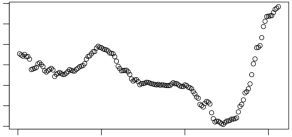
\includegraphics[width=0.3\textwidth]{work/picture/a_Swap1_1.png}};
    \node at(0.35,-0.15){\small 0};
    \node at(1.74,-0.15){\small 50};     
    \node at(3.2,-0.15){\small 100};
    \node at(4.65,-0.15){\small 150};   
    \node at(2.7,-0.8){\small month};
    \node at(2.63,2.8){ \hyperref[Swap41]{\textbf{Swap Rate for 1 Year Period}}};

    \node at(-0.2,0.2)[rotate=90]{\small 0};    
       \node at(-0.2,0.55)[rotate=90]{\small 1}; 
    \node at(-0.2,0.9)[rotate=90]{\small 2};  
    \node at(-0.2,1.25)[rotate=90]{\small 3};
    \node at(-0.2,1.6)[rotate=90]{\small 4};  
    \node at(-0.2,1.95)[rotate=90]{\small 5};
    \node at(-0.2,2.3)[rotate=90]{\small 6};  
    \node at(-1,1.2)[rotate=90]{\small Swap Rate in Percent};        

    
            \node[anchor=south west,inner sep=0] at (7,0) {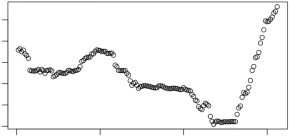
\includegraphics[width=0.3\textwidth]{work/picture/a_Yields.png}};
            \node at(9.5,2.8){ \hyperref[Yields42]{\textbf{Yields Rate for 1 Year Period}}};

    \node at(7+0.35,-0.15){\small 0};
    \node at(7+1.74,-0.15){\small 50};     
    \node at(7+3.2,-0.15){\small 100};
    \node at(7+4.65,-0.15){\small 150};   
    \node at(7+2.7,-0.8){\small Month};


     \node at(7-0.2,0.2)[rotate=90]{\small 0};    
       \node at(7+-0.2,0.55)[rotate=90]{\small 1}; 
    \node at(7+-0.2,0.9)[rotate=90]{\small 2};  
    \node at(7+-0.2,1.25)[rotate=90]{\small 3};
    \node at(7+-0.2,1.6)[rotate=90]{\small 4};  
    \node at(7+-0.2,1.95)[rotate=90]{\small 5};

     \node at(6,1.2)[rotate=90]{\small Yields Rate in Percent};   
        \end{tikzpicture}
    \caption{}
    %\label{Series2}
\end{figure}



\begin{figure}[H]
    \centering
        \begin{tikzpicture}[global scale = 1]
            \node[anchor=south west,inner sep=0] at (0,0) {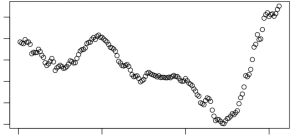
\includegraphics[width=0.3\textwidth]{work/picture/a_Swap2_1.png}};
    \node at(0.35,-0.15){\small 0};
    \node at(1.74,-0.15){\small 50};     
    \node at(3.2,-0.15){\small 100};
    \node at(4.65,-0.15){\small 150};   
    \node at(2.7,-0.8){\small month};
    \node at(2.63,2.8){\hyperref[Swap51]{\textbf{Swap Rate for 2 Year Period}}};

    \node at(-0.2,0.2)[rotate=90]{\small 0};    
       \node at(-0.2,0.6)[rotate=90]{\small 1}; 
    \node at(-0.2,0.95)[rotate=90]{\small 2};  
    \node at(-0.2,1.35)[rotate=90]{\small 3};
    \node at(-0.2,1.72)[rotate=90]{\small 4};  
    \node at(-0.2,2.1)[rotate=90]{\small 5};
    \node at(-1,1.2)[rotate=90]{\small Swap Rate in Percent};        

    
            \node[anchor=south west,inner sep=0] at (7,0) {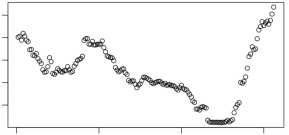
\includegraphics[width=0.3\textwidth]{work/picture/a_Yields2_2.png}};
            \node at(9.5,2.8){ \hyperref[Yields52]{\textbf{Yields Rate for 2 Year Period}}};

    \node at(7+0.35,-0.15){\small 0};
    \node at(7+1.74,-0.15){\small 50};     
    \node at(7+3.2,-0.15){\small 100};
    \node at(7+4.65,-0.15){\small 150};   
    \node at(7+2.7,-0.8){\small month};


     \node at(7-0.2,0.2+0.35)[rotate=90]{\small 1};    
       \node at(7+-0.2,0.55+0.36)[rotate=90]{\small 2}; 
    \node at(7+-0.2,0.9+0.41)[rotate=90]{\small 3};  
    \node at(7+-0.2,1.25+0.43)[rotate=90]{\small 4};
    \node at(7+-0.2,1.6+0.49)[rotate=90]{\small 5};  


     \node at(6,1.2)[rotate=90]{\small Yields Rate in Percent};   
        \end{tikzpicture}
    \caption{}
  %  \label{Series2}
\end{figure}


Test of filled variable

\begin{lstlisting}
        Augmented Dickey-Fuller Test
        
data: Yield.ts
Dickey-Fuller = -0.14344, Lag order = 5, p -value = 0.99 
alternative hypothesis: stationary    
\end{lstlisting}



\begin{figure}[H]
    \centering
        \begin{tikzpicture}[global scale = 1]
            \node[anchor=south west,inner sep=0] at (0,0) {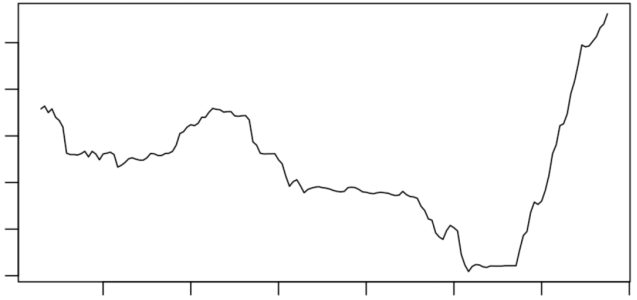
\includegraphics[width=0.8\textwidth]{work/picture/Yield_4.png}};
    \node at(13.3,-0.3){\small 2024};
    \node at(11.45,-0.3){\small 2022};     
    \node at(9.6,-0.3){\small 2020}; 
    \node at(7.75,-0.3){\small 2018}; 
    \node at(5.9,-0.3){\small 2016}; 
    \node at(4.05,-0.3){\small 2014}; 
    \node at(2.2,-0.3){\small 2012};    
    \node at(6.7,-1){\small month};   


    

    \node at(-0.3,0.5)[rotate=90]{\small 0};    
    \node at(-0.3,1.5)[rotate=90]{\small 1};   
    \node at(-0.3,2.5)[rotate=90]{\small 2};    
    \node at(-0.3,3.5)[rotate=90]{\small 3};   
    \node at(-0.3,4.5)[rotate=90]{\small 4};    
    \node at(-0.3,5.5)[rotate=90]{\small 5};   
    \node at(-1,3)[rotate=90]{\small Yield Rate in Percent};   
    
        \end{tikzpicture}
    \caption{\hyperref[Yields6]{Yield Rate for 1 Year Period}}
 %   \label{Series}
\end{figure}




\begin{figure}[H]
    \centering
        \begin{tikzpicture}[global scale = 1]
            \node[anchor=south west,inner sep=0] at (0,0) {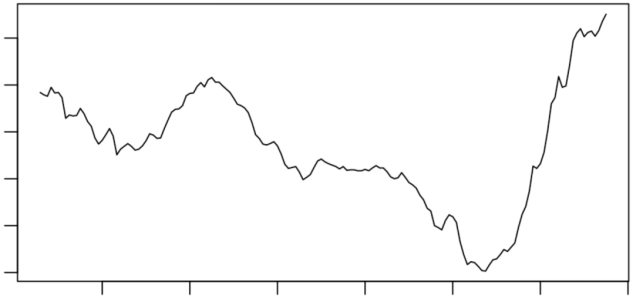
\includegraphics[width=0.8\textwidth]{work/picture/Swap.png}};
    \node at(13.3,-0.3){\small 2024};
    \node at(11.45,-0.3){\small 2022};     
    \node at(9.6,-0.3){\small 2020}; 
    \node at(7.75,-0.3){\small 2018}; 
    \node at(5.9,-0.3){\small 2016}; 
    \node at(4.05,-0.3){\small 2014}; 
    \node at(2.2,-0.3){\small 2012};    
    \node at(6.7,-1){\small month};   


    

    \node at(-0.3,0.5)[rotate=90]{\small 0};    
    \node at(-0.3,1.5)[rotate=90]{\small 1};   
    \node at(-0.3,2.5)[rotate=90]{\small 2};    
    \node at(-0.3,3.5)[rotate=90]{\small 3};   
    \node at(-0.3,4.5)[rotate=90]{\small 4};    
    \node at(-0.3,5.5)[rotate=90]{\small 5};   
    \node at(-1,3)[rotate=90]{\small Swap Rate in Percent};   
    
        \end{tikzpicture}
    \caption{\hyperref[Swap6]{Swap Rate for 2 Year Period}}
  %  \label{Series}
\end{figure}

\begin{figure}[H]
    \centering
        \begin{tikzpicture}[global scale = 1]
            \node[anchor=south west,inner sep=0] at (0,0) {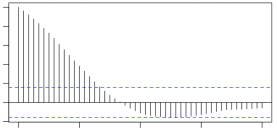
\includegraphics[width=0.3\textwidth]{work/picture/Series4_1.png}};
    \node at(0.35,-0.15){\small 0};
    \node at(1.49,-0.15){\small 1};     
    \node at(2.63,-0.15){\small 2};
    \node at(3.77,-0.15){\small 3};   
    \node at(4.92,-0.15){\small 4};
    \node at(2.63,-0.8){\small Lag};
    \node at(2.63,2.8){ \hyperref[Series71]{\textbf{Series Yield.ts}}};

    \node at(-0.2,0.2)[rotate=90]{\small -0.2};        
    \node at(-0.2,0.9)[rotate=90]{\small 0.2};  
    \node at(-0.2,1.6)[rotate=90]{\small 0.6};  
    \node at(-0.2,2.3)[rotate=90]{\small 1.0};  
    \node at(-1,1.2)[rotate=90]{\small ACF};        

    
            \node[anchor=south west,inner sep=0] at (7,0) {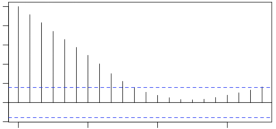
\includegraphics[width=0.3\textwidth]{work/picture/Series4_2.png}};
            \node at(9.5,2.8){ \hyperref[Series72]{\textbf{Series (Yield.ts-mean(Yield.ts))$^2$}}};

    \node at(7+0.4,-0.15){\small 0.0};     
    \node at(7+1.7,-0.15){\small 0.5};
    \node at(7+3,-0.15){\small 1.0};   
    \node at(7+4.3,-0.15){\small 1.5};
    \node at(7+2.63,-0.8){\small Lag};

    \node at(7+-0.2,0.2)[rotate=90]{\small -0.0};        
    \node at(7+-0.2,0.9)[rotate=90]{\small 0.2};  
    \node at(7+-0.2,1.6)[rotate=90]{\small 0.6};  
    \node at(7+-0.2,2.3)[rotate=90]{\small 1.0};  
    \node at(7+-1,1.2)[rotate=90]{\small ACF};   
        \end{tikzpicture}
    \caption{}
 %   \label{Series4}
\end{figure}




\begin{figure}[H]
    \centering
        \begin{tikzpicture}[global scale = 1]
            \node[anchor=south west,inner sep=0] at (0,0) {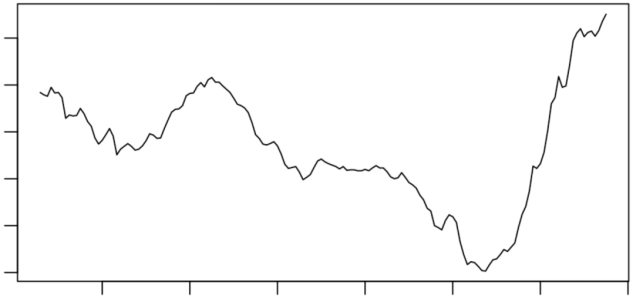
\includegraphics[width=0.8\textwidth]{work/picture/Swap.png}};
    \node at(13.3,-0.3){\small 2024};
    \node at(11.45,-0.3){\small 2022};     
    \node at(9.6,-0.3){\small 2020}; 
    \node at(7.75,-0.3){\small 2018}; 
    \node at(5.9,-0.3){\small 2016}; 
    \node at(4.05,-0.3){\small 2014}; 
    \node at(2.2,-0.3){\small 2012};    
    \node at(6.7,-1){\small Month};   


    

    \node at(-0.3,0.5)[rotate=90]{\small 0};    
    \node at(-0.3,1.5)[rotate=90]{\small 1};   
    \node at(-0.3,2.5)[rotate=90]{\small 2};    
    \node at(-0.3,3.5)[rotate=90]{\small 3};   
    \node at(-0.3,4.5)[rotate=90]{\small 4};    
    \node at(-0.3,5.5)[rotate=90]{\small 5};   
    \node at(-1,3)[rotate=90]{\small Swap Rate in Percent};   
    
        \end{tikzpicture}
    \caption{\hyperref[Swap8]{Swap Rate for 2 Year Period}}
  %  \label{Series}
\end{figure}

\begin{figure}[H]
    \centering
        \begin{tikzpicture}[global scale = 1]
            \node[anchor=south west,inner sep=0] at (0,0) {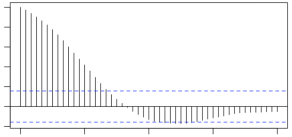
\includegraphics[width=0.3\textwidth]{work/picture/Series2_1.png}};
    \node at(0.35,-0.15){\small 0};
    \node at(1.49,-0.15){\small 1};     
    \node at(2.63,-0.15){\small 2};
    \node at(3.77,-0.15){\small 3};   
    \node at(4.92,-0.15){\small 4};
    \node at(2.63,-0.8){\small Lag};
    \node at(2.63,2.8){ \hyperref[Series10]{\textbf{Series swap.ts1}}};

    \node at(-0.2,0.2)[rotate=90]{\small -0.2};        
    \node at(-0.2,0.9)[rotate=90]{\small 0.2};  
    \node at(-0.2,1.6)[rotate=90]{\small 0.6};  
    \node at(-0.2,2.3)[rotate=90]{\small 1.0};  
    \node at(-1,1.2)[rotate=90]{\small ACF};        

    
            \node[anchor=south west,inner sep=0] at (7,0) {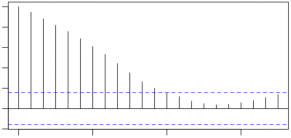
\includegraphics[width=0.3\textwidth]{work/picture/Series2_2.png}};
            \node at(9.5,2.8){ \hyperref[Series11]{\textbf{Series (swap.ts1-mean(swap.ts1))$^2$}}};

    \node at(7+0.4,-0.15){\small 0.0};     
    \node at(7+1.7,-0.15){\small 0.5};
    \node at(7+3,-0.15){\small 1.0};   
    \node at(7+4.3,-0.15){\small 1.5};
    \node at(7+2.63,-0.8){\small Lag};

    \node at(7+-0.2,0.2)[rotate=90]{\small -0.0};        
    \node at(7+-0.2,0.9)[rotate=90]{\small 0.2};  
    \node at(7+-0.2,1.6)[rotate=90]{\small 0.6};  
    \node at(7+-0.2,2.3)[rotate=90]{\small 1.0};  
    \node at(7+-1,1.2)[rotate=90]{\small ACF};   
        \end{tikzpicture}
    \caption{}
  %  \label{Series2}
\end{figure}

\begin{figure}[H]
    \centering
    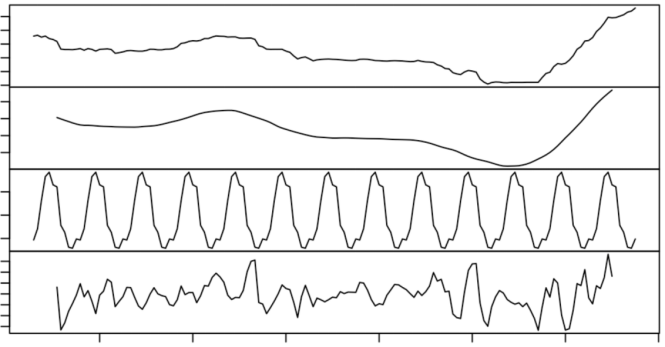
\includegraphics[width=0.8\textwidth]{work/picture/Decomposition3.png}
  \vspace{20pt}\caption{\hyperref[Decomposition3]{Decomposition of Additive Time Series}}
  %  \label{Decomposition}

    \begin{picture}(0,0)
        \put(0.37\textwidth,0.097\textwidth){\makebox(0,0)[lt]{\small{{2024}}}}
        \put(0.26\textwidth,0.097\textwidth){\makebox(0,0)[lt]{\small{{2022}}}}
        \put(0.15\textwidth,0.097\textwidth){\makebox(0,0)[lt]{\small{{2020}}}}
        \put(0.04\textwidth,0.097\textwidth){\makebox(0,0)[lt]{\small{{2018}}}}
        \put(-0.075\textwidth,0.097\textwidth){\makebox(0,0)[lt]{\small{{2016}}}}
        \put(-0.19\textwidth,0.097\textwidth){\makebox(0,0)[lt]{\small{{2014}}}}
        \put(-0.3\textwidth,0.097\textwidth){\makebox(0,0)[lt]{\small{{2012}}}}

        \put(-0.43\textwidth,0.15\textwidth){\makebox(0,0)[lt]{\rotatebox{90}{\small{-0.3}}}}
        \put(-0.43\textwidth,0.205\textwidth){\makebox(0,0)[lt]{\rotatebox{90}{\small{0.1}}}}
        \put(-0.43\textwidth,0.25\textwidth){\makebox(0,0)[lt]{\rotatebox{90}{\small{-0.05}}}}
        \put(-0.43\textwidth,0.33\textwidth){\makebox(0,0)[lt]{\rotatebox{90}{\small{0.05}}}}
        \put(-0.43\textwidth,0.35\textwidth){\makebox(0,0)[lt]{\rotatebox{90}{\small{1}}}}
        \put(-0.43\textwidth,0.39\textwidth){\makebox(0,0)[lt]{\rotatebox{90}{\small{3}}}}
        \put(-0.43\textwidth,0.43\textwidth){\makebox(0,0)[lt]{\rotatebox{90}{\small{0}}}}
        \put(-0.43\textwidth,0.46\textwidth){\makebox(0,0)[lt]{\rotatebox{90}{\small{2}}}}
        \put(-0.43\textwidth,0.498\textwidth){\makebox(0,0)[lt]{\rotatebox{90}{\small{4}}}}

        \put(-0.02\textwidth,0.07\textwidth){\makebox(0,0)[lt]{\textbf{Time}}}
        \put(-0.47\textwidth,0.47\textwidth){\makebox(0,0)[lt]{\rotatebox{90}{\textbf{Random Seasonal Trend Observed}}}}

    \end{picture}
\end{figure}


For 2 year period:
\begin{lstlisting}
        Augmented Dickey-Fuller Test
        
data: Yield.ts1
Dickey-Fuller = -0.29267, Lag order = 5, -value = 0.9899 
alternative hypothesis: stationary    
\end{lstlisting}




\begin{figure}[H]
    \centering
        \begin{tikzpicture}[global scale = 1]
            \node[anchor=south west,inner sep=0] at (0,0) {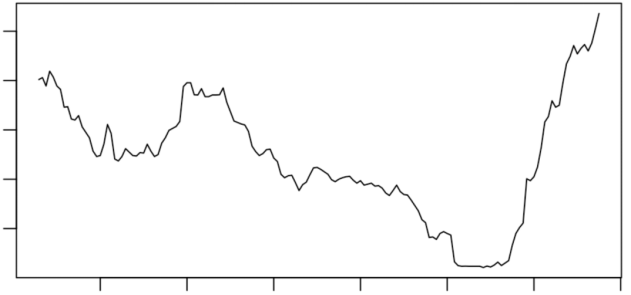
\includegraphics[width=0.8\textwidth]{work/picture/Yields5.png}};
    \node at(13.3,-0.3){\small 2024};
    \node at(11.45,-0.3){\small 2022};     
    \node at(9.6,-0.3){\small 2020}; 
    \node at(7.75,-0.3){\small 2018}; 
    \node at(5.9,-0.3){\small 2016}; 
    \node at(4.05,-0.3){\small 2014}; 
    \node at(2.2,-0.3){\small 2012};    
    \node at(6.7,-1){\small month};   

 
    \node at(-0.3,1.4)[rotate=90]{\small 1};   
    \node at(-0.3,2.5)[rotate=90]{\small 2};    
    \node at(-0.3,3.6)[rotate=90]{\small 3};   
    \node at(-0.3,4.7)[rotate=90]{\small 4};    
    \node at(-0.3,5.8)[rotate=90]{\small 5};   
    \node at(-1,3)[rotate=90]{\small Swap Rate in Percent};   
    
        \end{tikzpicture}
    \caption{\hyperref[Yield12]{Yield rate for 2 Year Period}}
  %  \label{Series}
\end{figure}





\begin{figure}[H]
    \centering
        \begin{tikzpicture}[global scale = 1]
            \node[anchor=south west,inner sep=0] at (0,0) {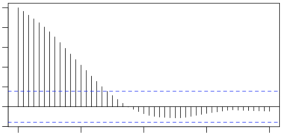
\includegraphics[width=0.3\textwidth]{work/picture/Series5_1.png}};
    \node at(0.35,-0.15){\small 0};
    \node at(1.49,-0.15){\small 1};     
    \node at(2.63,-0.15){\small 2};
    \node at(3.77,-0.15){\small 3};   
    \node at(4.92,-0.15){\small 4};
    \node at(2.63,-0.8){\small Lag};
    \node at(2.63,2.8){ \hyperref[Series13]{\textbf{Series Yield.ts1}}};

    \node at(-0.2,0.2)[rotate=90]{\small -0.2};        
    \node at(-0.2,0.9)[rotate=90]{\small 0.2};  
    \node at(-0.2,1.6)[rotate=90]{\small 0.6};  
    \node at(-0.2,2.3)[rotate=90]{\small 1.0};  
    \node at(-1,1.2)[rotate=90]{\small ACF};        

    
            \node[anchor=south west,inner sep=0] at (7,0) {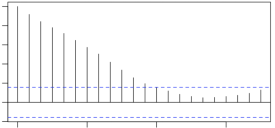
\includegraphics[width=0.3\textwidth]{work/picture/Series5_2.png}};
            \node at(9.5,2.8){ \hyperref[Series14]{\textbf{Series (Yield.ts1-mean(Yield.ts1))$^2$}}};

    \node at(7+0.4,-0.15){\small 0.0};     
    \node at(7+1.7,-0.15){\small 0.5};
    \node at(7+3,-0.15){\small 1.0};   
    \node at(7+4.3,-0.15){\small 1.5};
    \node at(7+2.63,-0.8){\small Lag};

    \node at(7+-0.2,0.2)[rotate=90]{\small -0.0};        
    \node at(7+-0.2,0.9)[rotate=90]{\small 0.2};  
    \node at(7+-0.2,1.6)[rotate=90]{\small 0.6};  
    \node at(7+-0.2,2.3)[rotate=90]{\small 1.0};  
    \node at(7+-1,1.2)[rotate=90]{\small ACF};   
        \end{tikzpicture}
    \caption{}
    \label{Series5}
\end{figure}


\begin{figure}[H]
    \centering
    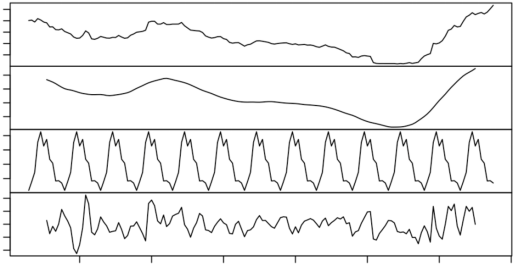
\includegraphics[width=0.8\textwidth]{work/picture/Decomposition4.png}
  \vspace{20pt}\caption{\hyperref[Decomposition4]{Decomposition of Additive Time Series}}
 %   \label{Decomposition}

    \begin{picture}(0,0)
        \put(0.365\textwidth,0.097\textwidth){\makebox(0,0)[lt]{\small{{2024}}}}
        \put(0.25\textwidth,0.097\textwidth){\makebox(0,0)[lt]{\small{{2022}}}}
        \put(0.145\textwidth,0.097\textwidth){\makebox(0,0)[lt]{\small{{2020}}}}
        \put(0.03\textwidth,0.097\textwidth){\makebox(0,0)[lt]{\small{{2018}}}}
        \put(-0.08\textwidth,0.097\textwidth){\makebox(0,0)[lt]{\small{{2016}}}}
        \put(-0.19\textwidth,0.097\textwidth){\makebox(0,0)[lt]{\small{{2014}}}}
        \put(-0.3\textwidth,0.097\textwidth){\makebox(0,0)[lt]{\small{{2012}}}}

        \put(-0.43\textwidth,0.15\textwidth){\makebox(0,0)[lt]{\rotatebox{90}{\small{-0.4}}}}
        \put(-0.43\textwidth,0.205\textwidth){\makebox(0,0)[lt]{\rotatebox{90}{\small{0.2}}}}
        \put(-0.43\textwidth,0.25\textwidth){\makebox(0,0)[lt]{\rotatebox{90}{\small{-0.05}}}}
        \put(-0.43\textwidth,0.33\textwidth){\makebox(0,0)[lt]{\rotatebox{90}{\small{0.10}}}}
        \put(-0.43\textwidth,0.345\textwidth){\makebox(0,0)[lt]{\rotatebox{90}{\small{1}}}}
        \put(-0.43\textwidth,0.39\textwidth){\makebox(0,0)[lt]{\rotatebox{90}{\small{3}}}}
        \put(-0.43\textwidth,0.44\textwidth){\makebox(0,0)[lt]{\rotatebox{90}{\small{1}}}}
        \put(-0.43\textwidth,0.47\textwidth){\makebox(0,0)[lt]{\rotatebox{90}{\small{3}}}}
        \put(-0.43\textwidth,0.51\textwidth){\makebox(0,0)[lt]{\rotatebox{90}{\small{5}}}}

        \put(-0.02\textwidth,0.07\textwidth){\makebox(0,0)[lt]{\textbf{Time}}}
        \put(-0.47\textwidth,0.47\textwidth){\makebox(0,0)[lt]{\rotatebox{90}{\textbf{Random Seasonal Trend Observed}}}}

    \end{picture}
\end{figure}


For the absent data preceding August 2010, we leveraged the interbank rate for predictions. The method resembled our previous predictions. Given the continuous data absence in 2009 – a tumultuous year post the financial crisis – a straightforward linear regression based on the interbank rate was deemed unsuitable.



\begin{figure}[H]
    \centering
        \begin{tikzpicture}[global scale = 1]
            \node[anchor=south west,inner sep=0] at (0,0) {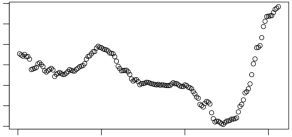
\includegraphics[width=0.3\textwidth]{work/picture/a_Swap1_1.png}};
    \node at(0.35,-0.15){\small 0};
    \node at(1.74,-0.15){\small 50};     
    \node at(3.2,-0.15){\small 100};
    \node at(4.65,-0.15){\small 150};   
    \node at(2.7,-0.8){\small month};
    \node at(2.63,2.8){ \hyperref[Swap15]{\textbf{Swap Rate for 1 Year Period}}};

    \node at(-0.2,0.2)[rotate=90]{\small 0};    
       \node at(-0.2,0.55)[rotate=90]{\small 1}; 
    \node at(-0.2,0.9)[rotate=90]{\small 2};  
    \node at(-0.2,1.25)[rotate=90]{\small 3};
    \node at(-0.2,1.6)[rotate=90]{\small 4};  
    \node at(-0.2,1.95)[rotate=90]{\small 5};
    \node at(-0.2,2.3)[rotate=90]{\small 6};  
    \node at(-1,1.2)[rotate=90]{\small Swap Rate in Percent};        

    
            \node[anchor=south west,inner sep=0] at (7,0) {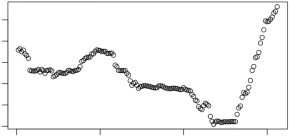
\includegraphics[width=0.3\textwidth]{work/picture/a_Yields.png}};
            \node at(9.5,2.8){ \hyperref[Yields15]{\textbf{Yields Rate for 1 Year Period}}};

    \node at(7+0.35,-0.15){\small 0};
    \node at(7+1.74,-0.15){\small 50};     
    \node at(7+3.2,-0.15){\small 100};
    \node at(7+4.65,-0.15){\small 150};   
    \node at(7+2.7,-0.8){\small month};


     \node at(7-0.2,0.2)[rotate=90]{\small 0};    
       \node at(7+-0.2,0.55)[rotate=90]{\small 1}; 
    \node at(7+-0.2,0.9)[rotate=90]{\small 2};  
    \node at(7+-0.2,1.25)[rotate=90]{\small 3};
    \node at(7+-0.2,1.6)[rotate=90]{\small 4};  
    \node at(7+-0.2,1.95)[rotate=90]{\small 5};

     \node at(6,1.2)[rotate=90]{\small Yields Rate in Percent};   
        \end{tikzpicture}
    \caption{}
    \label{Series2}
\end{figure}



\begin{figure}[H]
    \centering
        \begin{tikzpicture}[global scale = 1]
            \node[anchor=south west,inner sep=0] at (0,0) {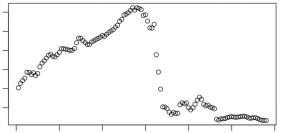
\includegraphics[width=0.3\textwidth]{work/picture/Interbank1.png}};
    \node at(0.3,-0.15){\small 0};
    \node at(1.075,-0.15){\small 20};
    \node at(1.85,-0.15){\small 40}; 
    \node at(2.625,-0.15){\small 60};
    \node at(3.4,-0.15){\small 80};
    \node at(4.175,-0.15){\small 100};
    \node at(4.95,-0.15){\small 120};   
    \node at(2.7,-0.8){\small month};
    \node at(2.63,2.8){ \hyperref[Interbank1]{\textbf{Interbank Rate for 1 Year Period}}};

    \node at(-0.2,0.4)[rotate=90]{\small 4};    
       \node at(-0.2,0.76)[rotate=90]{\small 5}; 
    \node at(-0.2,1.1)[rotate=90]{\small 6};  
    \node at(-0.2,1.47)[rotate=90]{\small 7};
    \node at(-0.2,1.82)[rotate=90]{\small 8};  
    \node at(-0.2,2.2)[rotate=90]{\small 9};
    \node at(-1,1.2)[rotate=90]{\small Swap Rate in Percent};        

    
            \node[anchor=south west,inner sep=0] at (7,0) {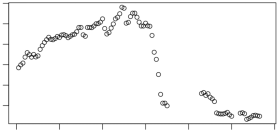
\includegraphics[width=0.3\textwidth]{work/picture/Yields5_2.png}};
            \node at(9.5,2.8){ \hyperref[Yields17]{\textbf{Yields Rate for 1 Year Period}}};

    \node at(7+0.3,-0.15){\small 0};
    \node at(7+1.075,-0.15){\small 20};
    \node at(7+1.85,-0.15){\small 40}; 
    \node at(7+2.625,-0.15){\small 60};
    \node at(7+3.4,-0.15){\small 80};
    \node at(7+4.175,-0.15){\small 100};
    \node at(7+4.95,-0.15){\small 120};   
    \node at(7+2.7,-0.8){\small month};



     \node at(7-0.2,0.2+0.32)[rotate=90]{\small 3};    
       \node at(7+-0.2,0.55+0.34)[rotate=90]{\small 4}; 
    \node at(7+-0.2,0.9+0.38)[rotate=90]{\small 5};  
    \node at(7+-0.2,1.25+0.39)[rotate=90]{\small 6};
    \node at(7+-0.2,1.6+0.43)[rotate=90]{\small 7};  
  \node at(7+-0.2,1.6+0.72)[rotate=90]{\small 8}; 

     \node at(6,1.2)[rotate=90]{\small Yields Rate in Percent};   
        \end{tikzpicture}
    \caption{}
    \label{Series2}
\end{figure}


After filled


\begin{figure}[H]
    \centering
        \begin{tikzpicture}[global scale = 1]
            \node[anchor=south west,inner sep=0] at (0,0) {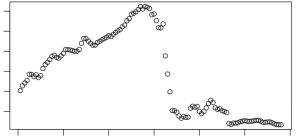
\includegraphics[width=0.3\textwidth]{work/picture/Interbank2.png}};
    \node at(0.3,-0.15){\small 0};
    \node at(1.075,-0.15){\small 20};
    \node at(1.85,-0.15){\small 40}; 
    \node at(2.625,-0.15){\small 60};
    \node at(3.4,-0.15){\small 80};
    \node at(4.175,-0.15){\small 100};
    \node at(4.95,-0.15){\small 120};   
    \node at(2.7,-0.8){\small month};
    \node at(2.63,2.8){ \hyperref[Interbank2]{\textbf{Interbank Rate for 1 Year Period}}};

    \node at(-0.2,0.4)[rotate=90]{\small 4};    
       \node at(-0.2,0.76)[rotate=90]{\small 5}; 
    \node at(-0.2,1.1)[rotate=90]{\small 6};  
    \node at(-0.2,1.47)[rotate=90]{\small 7};
    \node at(-0.2,1.82)[rotate=90]{\small 8};  
    \node at(-0.2,2.2)[rotate=90]{\small 9};
    \node at(-1,1.2)[rotate=90]{\small swap rate in percent};        

    
            \node[anchor=south west,inner sep=0] at (7,0) {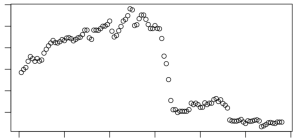
\includegraphics[width=0.3\textwidth]{work/picture/Yields6_2.png}};
            \node at(9.5,2.8){ \hyperref[Yields18]{\textbf{Yields Rate for 1 Year Period}}};

    \node at(7+0.3,-0.15){\small 0};
    \node at(7+1.075,-0.15){\small 20};
    \node at(7+1.85,-0.15){\small 40}; 
    \node at(7+2.625,-0.15){\small 60};
    \node at(7+3.4,-0.15){\small 80};
    \node at(7+4.175,-0.15){\small 100};
    \node at(7+4.95,-0.15){\small 120};   
    \node at(7+2.7,-0.8){\small Month};



     \node at(7-0.2,0.2+0.32)[rotate=90]{\small 3};    
       \node at(7+-0.2,0.55+0.34)[rotate=90]{\small 4}; 
    \node at(7+-0.2,0.9+0.38)[rotate=90]{\small 5};  
    \node at(7+-0.2,1.25+0.39)[rotate=90]{\small 6};
    \node at(7+-0.2,1.6+0.43)[rotate=90]{\small 7};  
  \node at(7+-0.2,1.6+0.72)[rotate=90]{\small 8}; 

     \node at(6,1.2)[rotate=90]{\small Yields Rate in Percent};   
        \end{tikzpicture}
    \caption{}
    \label{Series2}
\end{figure}




Final data:




\begin{figure}[H]
    \centering
        \begin{tikzpicture}[global scale = 1]
            \node[anchor=south west,inner sep=0] at (0,0) {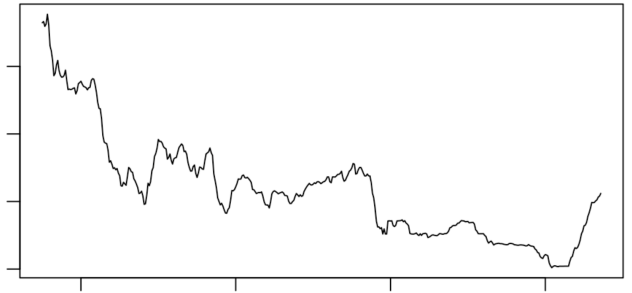
\includegraphics[width=0.8\textwidth]{work/picture/Yields7.png}};

    \node at(11.7,-0.3){\small 2020};  
    \node at(8.4,-0.3){\small 2010}; 
    \node at(5.1,-0.3){\small 2000}; 
    \node at(1.8,-0.3){\small 1990};    
    \node at(6.7,-1){\small Year};   


    \node at(-0.3,0.5)[rotate=90]{\small 0};    
    \node at(-0.3,1.95)[rotate=90]{\small 5};   
    \node at(-0.3,3.4)[rotate=90]{\small 10};    
    \node at(-0.3,4.85)[rotate=90]{\small 15};   

    \node at(-1,3)[rotate=90]{\small Yield Rate in Percent};   
    
        \end{tikzpicture}
    \caption{\hyperref[Yields19]{Yields Rate for 1 Year Period}}
%    \label{Series}
\end{figure}






\begin{figure}[H]
    \centering
        \begin{tikzpicture}[global scale = 1]
            \node[anchor=south west,inner sep=0] at (0,0) {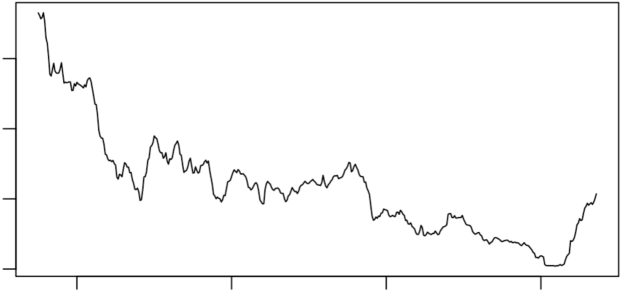
\includegraphics[width=0.8\textwidth]{work/picture/Yields8.png}};

    \node at(11.7,-0.3){\small 2020};  
    \node at(8.4,-0.3){\small 2010}; 
    \node at(5.1,-0.3){\small 2000}; 
    \node at(1.8,-0.3){\small 1990};    
    \node at(6.7,-1){\small year};   


    \node at(-0.3,0.5)[rotate=90]{\small 0};    
    \node at(-0.3,2.1)[rotate=90]{\small 5};   
    \node at(-0.3,3.7)[rotate=90]{\small 10};    
    \node at(-0.3,5.1)[rotate=90]{\small 15};   

    \node at(-1,3)[rotate=90]{\small yield rate in percent};   
    
        \end{tikzpicture}
    \caption{\hyperref[Yields20]{Yields rate for 2 Year Period}}
    \label{Series}
\end{figure}

\subsection{Conversion of Daily Data to Monthly Data:}

Certain datasets, such as the US yield data, were provided on a daily basis. To standardize this with our monthly datasets, I utilized Pivot Tables and the average function to transform these daily figures into monthly averages.

\printbibliography

\newpage

\pagenumbering{arabic}
\appendix

\section{Appendix A - Figure}
\begin{lstlisting}[language=R]

\end{lstlisting}



\begin{figure}[H]
    \centering
    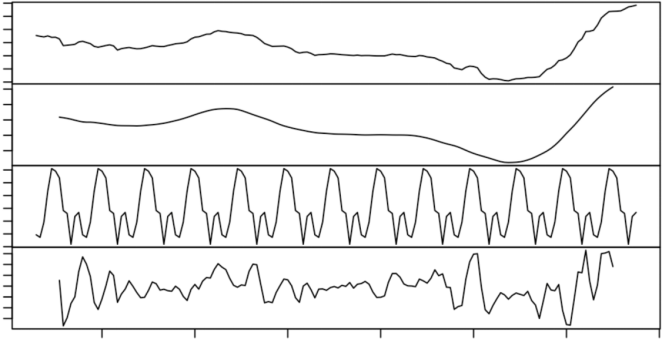
\includegraphics[width=0.8\textwidth]{work/picture/Decomposition.png}
  \vspace{20pt}\caption{Decomposition of Additive Time Series}
    \label{Decomposition1}

    \begin{picture}(0,0)
        \put(0.37\textwidth,0.097\textwidth){\makebox(0,0)[lt]{\small{{2024}}}}
        \put(0.26\textwidth,0.097\textwidth){\makebox(0,0)[lt]{\small{{2022}}}}
        \put(0.15\textwidth,0.097\textwidth){\makebox(0,0)[lt]{\small{{2020}}}}
        \put(0.04\textwidth,0.097\textwidth){\makebox(0,0)[lt]{\small{{2018}}}}
        \put(-0.07\textwidth,0.097\textwidth){\makebox(0,0)[lt]{\small{{2016}}}}
        \put(-0.18\textwidth,0.097\textwidth){\makebox(0,0)[lt]{\small{{2014}}}}
        \put(-0.29\textwidth,0.097\textwidth){\makebox(0,0)[lt]{\small{{2012}}}}

        \put(-0.43\textwidth,0.14\textwidth){\makebox(0,0)[lt]{\rotatebox{90}{\small{-0.3}}}}
        \put(-0.43\textwidth,0.19\textwidth){\makebox(0,0)[lt]{\rotatebox{90}{\small{0.1}}}}
        \put(-0.43\textwidth,0.23\textwidth){\makebox(0,0)[lt]{\rotatebox{90}{\small{-0.06}}}}
        \put(-0.43\textwidth,0.286\textwidth){\makebox(0,0)[lt]{\rotatebox{90}{\small{0.02}}}}
        \put(-0.43\textwidth,0.334\textwidth){\makebox(0,0)[lt]{\rotatebox{90}{\small{1}}}}
        \put(-0.43\textwidth,0.37\textwidth){\makebox(0,0)[lt]{\rotatebox{90}{\small{3}}}}
        \put(-0.43\textwidth,0.415\textwidth){\makebox(0,0)[lt]{\rotatebox{90}{\small{50}}}}
        \put(-0.43\textwidth,0.45\textwidth){\makebox(0,0)[lt]{\rotatebox{90}{\small{2}}}}
        \put(-0.43\textwidth,0.48\textwidth){\makebox(0,0)[lt]{\rotatebox{90}{\small{4}}}}
        \put(-0.43\textwidth,0.51\textwidth){\makebox(0,0)[lt]{\rotatebox{90}{\small{6}}}}

        \put(-0.02\textwidth,0.07\textwidth){\makebox(0,0)[lt]{\textbf{Time}}}
        \put(-0.47\textwidth,0.47\textwidth){\makebox(0,0)[lt]{\rotatebox{90}{\textbf{Random Seasonal Trend Observed}}}}

    \end{picture}
\end{figure}



\begin{figure}[H]
    \centering
        \begin{tikzpicture}[global scale = 1]
            \node[anchor=south west,inner sep=0] at (0,0) {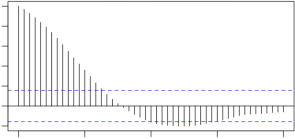
\includegraphics[width=0.3\textwidth]{work/picture/Series1.png}};
    \node at(0.35,-0.15){\small 0};
    \node at(1.49,-0.15){\small 1};     
    \node at(2.63,-0.15){\small 2};
    \node at(3.77,-0.15){\small 3};   
    \node at(4.92,-0.15){\small 4};
    \node at(2.63,-0.8){\small Lag};
    \node at(2.63,2.8){ \textbf{Series swap.ts}};

    \node at(-0.2,0.2)[rotate=90]{\small -0.2};        
    \node at(-0.2,0.9)[rotate=90]{\small 0.2};  
    \node at(-0.2,1.6)[rotate=90]{\small 0.6};  
    \node at(-0.2,2.3)[rotate=90]{\small 1.0};  
    \node at(-1,1.2)[rotate=90]{\small ACF};        
        \end{tikzpicture}
    \caption{Series swap.ts}
    \label{Series1}
\end{figure}


 \begin{figure}[H]
    \centering
        \begin{tikzpicture}[global scale = 1]   
            \node[anchor=south west,inner sep=0] at (7,0) {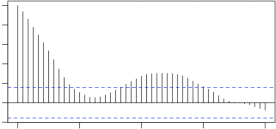
\includegraphics[width=0.3\textwidth]{work/picture/Series2.png}};
            \node at(9.5,2.8){ \textbf{Series (swap.ts-mean(swap.ts))$^2$}};
     \node at(7+0.35,-0.15){\small 0};
    \node at(7+1.49,-0.15){\small 1};     
    \node at(7+2.63,-0.15){\small 2};
    \node at(7+3.77,-0.15){\small 3};   
    \node at(7+4.92,-0.15){\small 4};
    \node at(7+2.63,-0.8){\small Lag};

    \node at(7+-0.2,0.2)[rotate=90]{\small -0.2};        
    \node at(7+-0.2,0.9)[rotate=90]{\small 0.2};  
    \node at(7+-0.2,1.6)[rotate=90]{\small 0.6};  
    \node at(7+-0.2,2.3)[rotate=90]{\small 1.0};  
    \node at(7+-1,1.2)[rotate=90]{\small ACF};   
        \end{tikzpicture}
    \caption{\textbf{Series (swap.ts-mean(swap.ts))$^2$}}
    \label{Series2}
\end{figure}







\begin{figure}[H]
    \centering
        \begin{tikzpicture}[global scale = 1]
            \node[anchor=south west,inner sep=0] at (0,0) {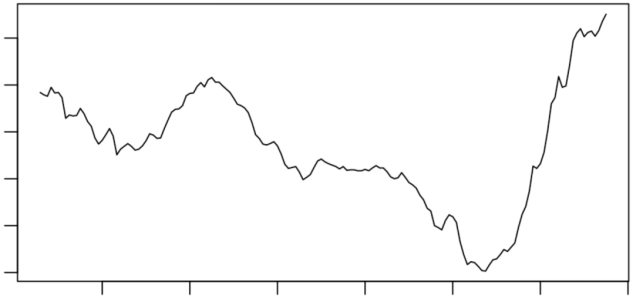
\includegraphics[width=0.8\textwidth]{work/picture/Swap.png}};
    \node at(13.3,-0.3){\small 2024};
    \node at(11.45,-0.3){\small 2022};     
    \node at(9.6,-0.3){\small 2020}; 
    \node at(7.75,-0.3){\small 2018}; 
    \node at(5.9,-0.3){\small 2016}; 
    \node at(4.05,-0.3){\small 2014}; 
    \node at(2.2,-0.3){\small 2012};    
    \node at(6.7,-1){\small Month};   


    

    \node at(-0.3,0.5)[rotate=90]{\small 0};    
    \node at(-0.3,1.5)[rotate=90]{\small 1};   
    \node at(-0.3,2.5)[rotate=90]{\small 2};    
    \node at(-0.3,3.5)[rotate=90]{\small 3};   
    \node at(-0.3,4.5)[rotate=90]{\small 4};    
    \node at(-0.3,5.5)[rotate=90]{\small 5};   
    \node at(-1,3)[rotate=90]{\small Swap Rate in Percent};   
    
        \end{tikzpicture}
    \caption{Swap Rate for 2 Year Period}
    \label{Swap}
\end{figure}





\begin{figure}[H]
    \centering
        \begin{tikzpicture}[global scale = 1]
            \node[anchor=south west,inner sep=0] at (0,0) {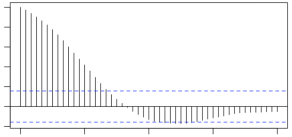
\includegraphics[width=0.3\textwidth]{work/picture/Series2_1.png}};
    \node at(0.35,-0.15){\small 0};
    \node at(1.49,-0.15){\small 1};     
    \node at(2.63,-0.15){\small 2};
    \node at(3.77,-0.15){\small 3};   
    \node at(4.92,-0.15){\small 4};
    \node at(2.63,-0.8){\small Lag};
    \node at(2.63,2.8){ \textbf{Series swap.ts1}};

    \node at(-0.2,0.2)[rotate=90]{\small -0.2};        
    \node at(-0.2,0.9)[rotate=90]{\small 0.2};  
    \node at(-0.2,1.6)[rotate=90]{\small 0.6};  
    \node at(-0.2,2.3)[rotate=90]{\small 1.0};  
    \node at(-1,1.2)[rotate=90]{\small ACF};        
        \end{tikzpicture}
    \caption{}
    \label{Series21}
\end{figure}

\begin{figure}[H]
    \centering
        \begin{tikzpicture}[global scale = 1]    
            \node[anchor=south west,inner sep=0] at (7,0) {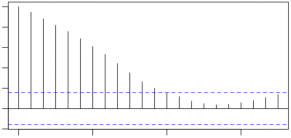
\includegraphics[width=0.3\textwidth]{work/picture/Series2_2.png}};
            \node at(9.5,2.8){ \textbf{Series (swap.ts1-mean(swap.ts1))$^2$}};

    \node at(7+0.4,-0.15){\small 0.0};     
    \node at(7+1.7,-0.15){\small 0.5};
    \node at(7+3,-0.15){\small 1.0};   
    \node at(7+4.3,-0.15){\small 1.5};
    \node at(7+2.63,-0.8){\small Lag};

    \node at(7+-0.2,0.2)[rotate=90]{\small -0.0};        
    \node at(7+-0.2,0.9)[rotate=90]{\small 0.2};  
    \node at(7+-0.2,1.6)[rotate=90]{\small 0.6};  
    \node at(7+-0.2,2.3)[rotate=90]{\small 1.0};  
    \node at(7+-1,1.2)[rotate=90]{\small ACF};   
        \end{tikzpicture}
    \caption{}
    \label{Series22}
\end{figure}




\begin{figure}[H]
    \centering
    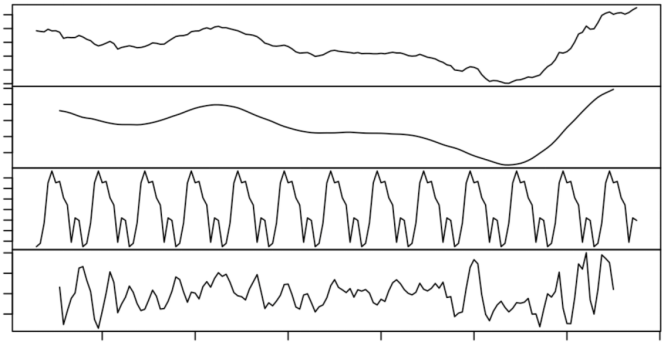
\includegraphics[width=0.8\textwidth]{work/picture/Decomposition2.png}
  \vspace{20pt}\caption{Decomposition of Additive Time Series}
    \label{Decomposition2}

    \begin{picture}(0,0)
        \put(0.37\textwidth,0.097\textwidth){\makebox(0,0)[lt]{\small{{2024}}}}
        \put(0.26\textwidth,0.097\textwidth){\makebox(0,0)[lt]{\small{{2022}}}}
        \put(0.15\textwidth,0.097\textwidth){\makebox(0,0)[lt]{\small{{2020}}}}
        \put(0.04\textwidth,0.097\textwidth){\makebox(0,0)[lt]{\small{{2018}}}}
        \put(-0.075\textwidth,0.097\textwidth){\makebox(0,0)[lt]{\small{{2016}}}}
        \put(-0.19\textwidth,0.097\textwidth){\makebox(0,0)[lt]{\small{{2014}}}}
        \put(-0.3\textwidth,0.097\textwidth){\makebox(0,0)[lt]{\small{{2012}}}}

        \put(-0.43\textwidth,0.16\textwidth){\makebox(0,0)[lt]{\rotatebox{90}{\small{-0.2}}}}
        \put(-0.43\textwidth,0.205\textwidth){\makebox(0,0)[lt]{\rotatebox{90}{\small{0.2}}}}
        \put(-0.43\textwidth,0.25\textwidth){\makebox(0,0)[lt]{\rotatebox{90}{\small{-0.06}}}}
        \put(-0.43\textwidth,0.306\textwidth){\makebox(0,0)[lt]{\rotatebox{90}{\small{0.02}}}}
        \put(-0.43\textwidth,0.348\textwidth){\makebox(0,0)[lt]{\rotatebox{90}{\small{1}}}}
        \put(-0.43\textwidth,0.383\textwidth){\makebox(0,0)[lt]{\rotatebox{90}{\small{3}}}}
        \put(-0.43\textwidth,0.425\textwidth){\makebox(0,0)[lt]{\rotatebox{90}{\small{50}}}}
        \put(-0.43\textwidth,0.46\textwidth){\makebox(0,0)[lt]{\rotatebox{90}{\small{2}}}}
        \put(-0.43\textwidth,0.49\textwidth){\makebox(0,0)[lt]{\rotatebox{90}{\small{4}}}}

        \put(-0.02\textwidth,0.07\textwidth){\makebox(0,0)[lt]{\textbf{Time}}}
        \put(-0.47\textwidth,0.47\textwidth){\makebox(0,0)[lt]{\rotatebox{90}{\textbf{random seasonal trend observed}}}}

    \end{picture}
\end{figure}





\begin{figure}[H]
    \centering
        \begin{tikzpicture}[global scale = 1]
            \node[anchor=south west,inner sep=0] at (0,0) {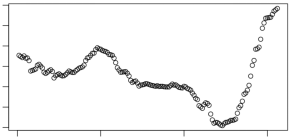
\includegraphics[width=0.3\textwidth]{work/picture/Swap2_1.png}};
    \node at(0.35,-0.15){\small 0};
    \node at(1.74,-0.15){\small 50};     
    \node at(3.2,-0.15){\small 100};
    \node at(4.65,-0.15){\small 150};   
    \node at(2.7,-0.8){\small Month};
    \node at(2.63,2.8){ \textbf{Swap Rate for 1 Year Period}};

    \node at(-0.2,0.2)[rotate=90]{\small 0};    
       \node at(-0.2,0.55)[rotate=90]{\small 1}; 
    \node at(-0.2,0.9)[rotate=90]{\small 2};  
    \node at(-0.2,1.25)[rotate=90]{\small 3};
    \node at(-0.2,1.6)[rotate=90]{\small 4};  
    \node at(-0.2,1.95)[rotate=90]{\small 5};
    \node at(-0.2,2.3)[rotate=90]{\small 6};  
    \node at(-1,1.2)[rotate=90]{\small Swap Rate in Percent};        
        \end{tikzpicture}
    \caption{}
    \label{Swap21}
\end{figure}

\begin{figure}[H]
    \centering
        \begin{tikzpicture}[global scale = 1]    
            \node[anchor=south west,inner sep=0] at (7,0) {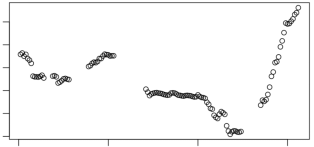
\includegraphics[width=0.3\textwidth]{work/picture/Yields.png}};
            \node at(9.5,2.8){ \textbf{Yields Rate for 1 Year Period}};

    \node at(7+0.35,-0.15){\small 0};
    \node at(7+1.74,-0.15){\small 50};     
    \node at(7+3.2,-0.15){\small 100};
    \node at(7+4.65,-0.15){\small 150};   
    \node at(7+2.7,-0.8){\small month};


     \node at(7-0.2,0.2)[rotate=90]{\small 0};    
       \node at(7+-0.2,0.55)[rotate=90]{\small 1}; 
    \node at(7+-0.2,0.9)[rotate=90]{\small 2};  
    \node at(7+-0.2,1.25)[rotate=90]{\small 3};
    \node at(7+-0.2,1.6)[rotate=90]{\small 4};  
    \node at(7+-0.2,1.95)[rotate=90]{\small 5};

     \node at(6,1.2)[rotate=90]{\small yields rate in percent};   
        \end{tikzpicture}
    \caption{}
    \label{Yields2}
\end{figure}



\begin{figure}[H]
    \centering
        \begin{tikzpicture}[global scale = 1]
            \node[anchor=south west,inner sep=0] at (0,0) {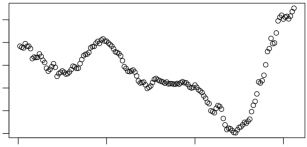
\includegraphics[width=0.3\textwidth]{work/picture/Swap3_1.png}};
    \node at(0.35,-0.15){\small 0};
    \node at(1.74,-0.15){\small 50};     
    \node at(3.2,-0.15){\small 100};
    \node at(4.65,-0.15){\small 150};   
    \node at(2.7,-0.8){\small month};
    \node at(2.63,2.8){ \textbf{Swap Rate for 2 Year Period}};

    \node at(-0.2,0.2)[rotate=90]{\small 0};    
       \node at(-0.2,0.6)[rotate=90]{\small 1}; 
    \node at(-0.2,0.95)[rotate=90]{\small 2};  
    \node at(-0.2,1.35)[rotate=90]{\small 3};
    \node at(-0.2,1.72)[rotate=90]{\small 4};  
    \node at(-0.2,2.1)[rotate=90]{\small 5};
    \node at(-1,1.2)[rotate=90]{\small swap rate in percent};        
        \end{tikzpicture}
    \caption{}
    \label{Swap31}
\end{figure}
    
 
\begin{figure}[H]
    \centering
        \begin{tikzpicture}[global scale = 1]
        \node[anchor=south west,inner sep=0] at (7,0) {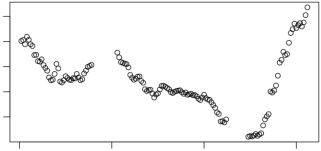
\includegraphics[width=0.3\textwidth]{work/picture/Yield3_2.png}};
            \node at(9.5,2.8){ \textbf{Yields Rate for 2 Year Period}};

    \node at(7+0.35,-0.15){\small 0};
    \node at(7+1.74,-0.15){\small 50};     
    \node at(7+3.2,-0.15){\small 100};
    \node at(7+4.65,-0.15){\small 150};   
    \node at(7+2.7,-0.8){\small month};


     \node at(7-0.2,0.2+0.35)[rotate=90]{\small 1};    
       \node at(7+-0.2,0.55+0.36)[rotate=90]{\small 2}; 
    \node at(7+-0.2,0.9+0.41)[rotate=90]{\small 3};  
    \node at(7+-0.2,1.25+0.43)[rotate=90]{\small 4};
    \node at(7+-0.2,1.6+0.49)[rotate=90]{\small 5};  


     \node at(6,1.2)[rotate=90]{\small yields rate in percent};   
        \end{tikzpicture}
    \caption{}
    \label{Yields32}
\end{figure}




\begin{figure}[H]
    \centering
        \begin{tikzpicture}[global scale = 1]
            \node[anchor=south west,inner sep=0] at (0,0) {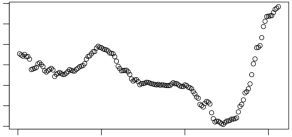
\includegraphics[width=0.3\textwidth]{work/picture/a_Swap1_1.png}};
    \node at(0.35,-0.15){\small 0};
    \node at(1.74,-0.15){\small 50};     
    \node at(3.2,-0.15){\small 100};
    \node at(4.65,-0.15){\small 150};   
    \node at(2.7,-0.8){\small month};
    \node at(2.63,2.8){ \textbf{Swap Rate for 1 Year Period}};

    \node at(-0.2,0.2)[rotate=90]{\small 0};    
       \node at(-0.2,0.55)[rotate=90]{\small 1}; 
    \node at(-0.2,0.9)[rotate=90]{\small 2};  
    \node at(-0.2,1.25)[rotate=90]{\small 3};
    \node at(-0.2,1.6)[rotate=90]{\small 4};  
    \node at(-0.2,1.95)[rotate=90]{\small 5};
    \node at(-0.2,2.3)[rotate=90]{\small 6};  
    \node at(-1,1.2)[rotate=90]{\small swap rate in percent};        
        \end{tikzpicture}
    \caption{}
    \label{Swap41}
\end{figure}

\begin{figure}[H]
    \centering
        \begin{tikzpicture}[global scale = 1]    
            \node[anchor=south west,inner sep=0] at (7,0) {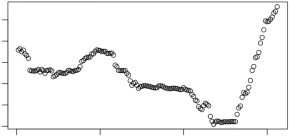
\includegraphics[width=0.3\textwidth]{work/picture/a_Yields.png}};
            \node at(9.5,2.8){ \textbf{Yields Rate for 1 Year Period}};

    \node at(7+0.35,-0.15){\small 0};
    \node at(7+1.74,-0.15){\small 50};     
    \node at(7+3.2,-0.15){\small 100};
    \node at(7+4.65,-0.15){\small 150};   
    \node at(7+2.7,-0.8){\small month};


     \node at(7-0.2,0.2)[rotate=90]{\small 0};    
       \node at(7+-0.2,0.55)[rotate=90]{\small 1}; 
    \node at(7+-0.2,0.9)[rotate=90]{\small 2};  
    \node at(7+-0.2,1.25)[rotate=90]{\small 3};
    \node at(7+-0.2,1.6)[rotate=90]{\small 4};  
    \node at(7+-0.2,1.95)[rotate=90]{\small 5};

     \node at(6,1.2)[rotate=90]{\small yields rate in percent};   
        \end{tikzpicture}
    \caption{}
    \label{Yields42}
\end{figure}




\begin{figure}[H]
    \centering
        \begin{tikzpicture}[global scale = 1]
            \node[anchor=south west,inner sep=0] at (0,0) {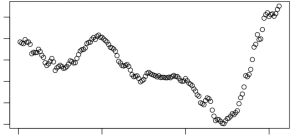
\includegraphics[width=0.3\textwidth]{work/picture/a_Swap2_1.png}};
    \node at(0.35,-0.15){\small 0};
    \node at(1.74,-0.15){\small 50};     
    \node at(3.2,-0.15){\small 100};
    \node at(4.65,-0.15){\small 150};   
    \node at(2.7,-0.8){\small month};
    \node at(2.63,2.8){ \textbf{Swap Rate for 2 Year Period}};

    \node at(-0.2,0.2)[rotate=90]{\small 0};    
       \node at(-0.2,0.6)[rotate=90]{\small 1}; 
    \node at(-0.2,0.95)[rotate=90]{\small 2};  
    \node at(-0.2,1.35)[rotate=90]{\small 3};
    \node at(-0.2,1.72)[rotate=90]{\small 4};  
    \node at(-0.2,2.1)[rotate=90]{\small 5};
    \node at(-1,1.2)[rotate=90]{\small swap rate in percent};        
        \end{tikzpicture}
    \caption{}
    \label{Swap51}
\end{figure}

  \begin{figure}[H]
    \centering
        \begin{tikzpicture}[global scale = 1]  
            \node[anchor=south west,inner sep=0] at (7,0) {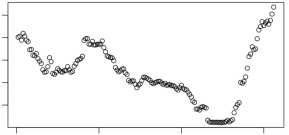
\includegraphics[width=0.3\textwidth]{work/picture/a_Yields2_2.png}};
            \node at(9.5,2.8){ \textbf{Yields Rate for 2 Year Period}};

    \node at(7+0.35,-0.15){\small 0};
    \node at(7+1.74,-0.15){\small 50};     
    \node at(7+3.2,-0.15){\small 100};
    \node at(7+4.65,-0.15){\small 150};   
    \node at(7+2.7,-0.8){\small month};


     \node at(7-0.2,0.2+0.35)[rotate=90]{\small 1};    
       \node at(7+-0.2,0.55+0.36)[rotate=90]{\small 2}; 
    \node at(7+-0.2,0.9+0.41)[rotate=90]{\small 3};  
    \node at(7+-0.2,1.25+0.43)[rotate=90]{\small 4};
    \node at(7+-0.2,1.6+0.49)[rotate=90]{\small 5};  


     \node at(6,1.2)[rotate=90]{\small yields rate in percent};   
        \end{tikzpicture}
    \caption{}
  %  \label{Yields52}
\end{figure}





\begin{figure}[H]
    \centering
        \begin{tikzpicture}[global scale = 1]
            \node[anchor=south west,inner sep=0] at (0,0) {\includegraphics[width=0.8\textwidth]{work/picture/Yield_4.png}};
    \node at(13.3,-0.3){\small 2024};
    \node at(11.45,-0.3){\small 2022};     
    \node at(9.6,-0.3){\small 2020}; 
    \node at(7.75,-0.3){\small 2018}; 
    \node at(5.9,-0.3){\small 2016}; 
    \node at(4.05,-0.3){\small 2014}; 
    \node at(2.2,-0.3){\small 2012};    
    \node at(6.7,-1){\small month};   


    

    \node at(-0.3,0.5)[rotate=90]{\small 0};    
    \node at(-0.3,1.5)[rotate=90]{\small 1};   
    \node at(-0.3,2.5)[rotate=90]{\small 2};    
    \node at(-0.3,3.5)[rotate=90]{\small 3};   
    \node at(-0.3,4.5)[rotate=90]{\small 4};    
    \node at(-0.3,5.5)[rotate=90]{\small 5};   
    \node at(-1,3)[rotate=90]{\small yield rate in percent};   
    
        \end{tikzpicture}
    \caption{Yield rate for 1 Year Period}
    \label{Yields6}
\end{figure}



\begin{figure}[H]
    \centering
        \begin{tikzpicture}[global scale = 1]
            \node[anchor=south west,inner sep=0] at (0,0) {\includegraphics[width=0.8\textwidth]{work/picture/Swap.png}};
    \node at(13.3,-0.3){\small 2024};
    \node at(11.45,-0.3){\small 2022};     
    \node at(9.6,-0.3){\small 2020}; 
    \node at(7.75,-0.3){\small 2018}; 
    \node at(5.9,-0.3){\small 2016}; 
    \node at(4.05,-0.3){\small 2014}; 
    \node at(2.2,-0.3){\small 2012};    
    \node at(6.7,-1){\small month};   


    

    \node at(-0.3,0.5)[rotate=90]{\small 0};    
    \node at(-0.3,1.5)[rotate=90]{\small 1};   
    \node at(-0.3,2.5)[rotate=90]{\small 2};    
    \node at(-0.3,3.5)[rotate=90]{\small 3};   
    \node at(-0.3,4.5)[rotate=90]{\small 4};    
    \node at(-0.3,5.5)[rotate=90]{\small 5};   
    \node at(-1,3)[rotate=90]{\small swap rate in percent};   
    
        \end{tikzpicture}
    \caption{Swap rate for 2 Year Period}
    \label{Swap6}
\end{figure}



\begin{figure}[H]
    \centering
        \begin{tikzpicture}[global scale = 1]
            \node[anchor=south west,inner sep=0] at (0,0) {\includegraphics[width=0.3\textwidth]{work/picture/Series4_1.png}};
    \node at(0.35,-0.15){\small 0};
    \node at(1.49,-0.15){\small 1};     
    \node at(2.63,-0.15){\small 2};
    \node at(3.77,-0.15){\small 3};   
    \node at(4.92,-0.15){\small 4};
    \node at(2.63,-0.8){\small Lag};
    \node at(2.63,2.8){ \textbf{Series Yield.ts}};

    \node at(-0.2,0.2)[rotate=90]{\small -0.2};        
    \node at(-0.2,0.9)[rotate=90]{\small 0.2};  
    \node at(-0.2,1.6)[rotate=90]{\small 0.6};  
    \node at(-0.2,2.3)[rotate=90]{\small 1.0};  
    \node at(-1,1.2)[rotate=90]{\small ACF};        
        \end{tikzpicture}
    \caption{}
    \label{Series71}
\end{figure}

   \begin{figure}[H]
    \centering
        \begin{tikzpicture}[global scale = 1] 
            \node[anchor=south west,inner sep=0] at (7,0) {\includegraphics[width=0.3\textwidth]{work/picture/Series4_2.png}};
            \node at(9.5,2.8){ \textbf{Series (Yield.ts-mean(Yield.ts))$^2$}};

    \node at(7+0.4,-0.15){\small 0.0};     
    \node at(7+1.7,-0.15){\small 0.5};
    \node at(7+3,-0.15){\small 1.0};   
    \node at(7+4.3,-0.15){\small 1.5};
    \node at(7+2.63,-0.8){\small Lag};

    \node at(7+-0.2,0.2)[rotate=90]{\small -0.0};        
    \node at(7+-0.2,0.9)[rotate=90]{\small 0.2};  
    \node at(7+-0.2,1.6)[rotate=90]{\small 0.6};  
    \node at(7+-0.2,2.3)[rotate=90]{\small 1.0};  
    \node at(7+-1,1.2)[rotate=90]{\small ACF};   
        \end{tikzpicture}
    \caption{}
    \label{Series72}
\end{figure}


\begin{figure}[H]
    \centering
        \begin{tikzpicture}[global scale = 1]
            \node[anchor=south west,inner sep=0] at (0,0) {\includegraphics[width=0.8\textwidth]{work/picture/Swap.png}};
    \node at(13.3,-0.3){\small 2024};
    \node at(11.45,-0.3){\small 2022};     
    \node at(9.6,-0.3){\small 2020}; 
    \node at(7.75,-0.3){\small 2018}; 
    \node at(5.9,-0.3){\small 2016}; 
    \node at(4.05,-0.3){\small 2014}; 
    \node at(2.2,-0.3){\small 2012};    
    \node at(6.7,-1){\small month};   


    

    \node at(-0.3,0.5)[rotate=90]{\small 0};    
    \node at(-0.3,1.5)[rotate=90]{\small 1};   
    \node at(-0.3,2.5)[rotate=90]{\small 2};    
    \node at(-0.3,3.5)[rotate=90]{\small 3};   
    \node at(-0.3,4.5)[rotate=90]{\small 4};    
    \node at(-0.3,5.5)[rotate=90]{\small 5};   
    \node at(-1,3)[rotate=90]{\small swap rate in percent};   
    
        \end{tikzpicture}
    \caption{Swap rate for 2 Year Period}
    \label{Swap8}
\end{figure}



\begin{figure}[H]
    \centering
        \begin{tikzpicture}[global scale = 1]
            \node[anchor=south west,inner sep=0] at (0,0) {\includegraphics[width=0.3\textwidth]{work/picture/Series2_1.png}};
    \node at(0.35,-0.15){\small 0};
    \node at(1.49,-0.15){\small 1};     
    \node at(2.63,-0.15){\small 2};
    \node at(3.77,-0.15){\small 3};   
    \node at(4.92,-0.15){\small 4};
    \node at(2.63,-0.8){\small Lag};
    \node at(2.63,2.8){ \textbf{Series swap.ts1}};

    \node at(-0.2,0.2)[rotate=90]{\small -0.2};        
    \node at(-0.2,0.9)[rotate=90]{\small 0.2};  
    \node at(-0.2,1.6)[rotate=90]{\small 0.6};  
    \node at(-0.2,2.3)[rotate=90]{\small 1.0};  
    \node at(-1,1.2)[rotate=90]{\small ACF};        
        \end{tikzpicture}
    \caption{}
    \label{Series10}
\end{figure}


\begin{figure}[H]
    \centering
        \begin{tikzpicture}[global scale = 1]    
            \node[anchor=south west,inner sep=0] at (7,0) {\includegraphics[width=0.3\textwidth]{work/picture/Series2_2.png}};
            \node at(9.5,2.8){ \textbf{Series (swap.ts1-mean(swap.ts1))$^2$}};

    \node at(7+0.4,-0.15){\small 0.0};     
    \node at(7+1.7,-0.15){\small 0.5};
    \node at(7+3,-0.15){\small 1.0};   
    \node at(7+4.3,-0.15){\small 1.5};
    \node at(7+2.63,-0.8){\small Lag};

    \node at(7+-0.2,0.2)[rotate=90]{\small -0.0};        
    \node at(7+-0.2,0.9)[rotate=90]{\small 0.2};  
    \node at(7+-0.2,1.6)[rotate=90]{\small 0.6};  
    \node at(7+-0.2,2.3)[rotate=90]{\small 1.0};  
    \node at(7+-1,1.2)[rotate=90]{\small ACF};   
        \end{tikzpicture}
    \caption{}
    \label{Series11}
\end{figure}





\begin{figure}[H]
    \centering
    \includegraphics[width=0.8\textwidth]{work/picture/Decomposition3.png}
  \vspace{20pt}\caption{Decomposition of additive time series}
    \label{Decomposition3}

    \begin{picture}(0,0)
        \put(0.37\textwidth,0.097\textwidth){\makebox(0,0)[lt]{\small{{2024}}}}
        \put(0.26\textwidth,0.097\textwidth){\makebox(0,0)[lt]{\small{{2022}}}}
        \put(0.15\textwidth,0.097\textwidth){\makebox(0,0)[lt]{\small{{2020}}}}
        \put(0.04\textwidth,0.097\textwidth){\makebox(0,0)[lt]{\small{{2018}}}}
        \put(-0.075\textwidth,0.097\textwidth){\makebox(0,0)[lt]{\small{{2016}}}}
        \put(-0.19\textwidth,0.097\textwidth){\makebox(0,0)[lt]{\small{{2014}}}}
        \put(-0.3\textwidth,0.097\textwidth){\makebox(0,0)[lt]{\small{{2012}}}}

        \put(-0.43\textwidth,0.15\textwidth){\makebox(0,0)[lt]{\rotatebox{90}{\small{-0.3}}}}
        \put(-0.43\textwidth,0.205\textwidth){\makebox(0,0)[lt]{\rotatebox{90}{\small{0.1}}}}
        \put(-0.43\textwidth,0.25\textwidth){\makebox(0,0)[lt]{\rotatebox{90}{\small{-0.05}}}}
        \put(-0.43\textwidth,0.33\textwidth){\makebox(0,0)[lt]{\rotatebox{90}{\small{0.05}}}}
        \put(-0.43\textwidth,0.35\textwidth){\makebox(0,0)[lt]{\rotatebox{90}{\small{1}}}}
        \put(-0.43\textwidth,0.39\textwidth){\makebox(0,0)[lt]{\rotatebox{90}{\small{3}}}}
        \put(-0.43\textwidth,0.43\textwidth){\makebox(0,0)[lt]{\rotatebox{90}{\small{0}}}}
        \put(-0.43\textwidth,0.46\textwidth){\makebox(0,0)[lt]{\rotatebox{90}{\small{2}}}}
        \put(-0.43\textwidth,0.498\textwidth){\makebox(0,0)[lt]{\rotatebox{90}{\small{4}}}}

        \put(-0.02\textwidth,0.07\textwidth){\makebox(0,0)[lt]{\textbf{Time}}}
        \put(-0.47\textwidth,0.47\textwidth){\makebox(0,0)[lt]{\rotatebox{90}{\textbf{random seasonal trend observed}}}}

    \end{picture}
\end{figure}


\begin{figure}[H]
    \centering
        \begin{tikzpicture}[global scale = 1]
            \node[anchor=south west,inner sep=0] at (0,0) {\includegraphics[width=0.8\textwidth]{work/picture/Yields5.png}};
    \node at(13.3,-0.3){\small 2024};
    \node at(11.45,-0.3){\small 2022};     
    \node at(9.6,-0.3){\small 2020}; 
    \node at(7.75,-0.3){\small 2018}; 
    \node at(5.9,-0.3){\small 2016}; 
    \node at(4.05,-0.3){\small 2014}; 
    \node at(2.2,-0.3){\small 2012};    
    \node at(6.7,-1){\small month};   

 
    \node at(-0.3,1.4)[rotate=90]{\small 1};   
    \node at(-0.3,2.5)[rotate=90]{\small 2};    
    \node at(-0.3,3.6)[rotate=90]{\small 3};   
    \node at(-0.3,4.7)[rotate=90]{\small 4};    
    \node at(-0.3,5.8)[rotate=90]{\small 5};   
    \node at(-1,3)[rotate=90]{\small swap rate in percent};   
    
        \end{tikzpicture}
    \caption{Yield rate for 2 Year Period}
    \label{Yield12}
\end{figure}


\begin{figure}[H]
    \centering
        \begin{tikzpicture}[global scale = 1]
            \node[anchor=south west,inner sep=0] at (0,0) {\includegraphics[width=0.3\textwidth]{work/picture/Series5_1.png}};
    \node at(0.35,-0.15){\small 0};
    \node at(1.49,-0.15){\small 1};     
    \node at(2.63,-0.15){\small 2};
    \node at(3.77,-0.15){\small 3};   
    \node at(4.92,-0.15){\small 4};
    \node at(2.63,-0.8){\small Lag};
    \node at(2.63,2.8){ \textbf{Series Yield.ts1}};

    \node at(-0.2,0.2)[rotate=90]{\small -0.2};        
    \node at(-0.2,0.9)[rotate=90]{\small 0.2};  
    \node at(-0.2,1.6)[rotate=90]{\small 0.6};  
    \node at(-0.2,2.3)[rotate=90]{\small 1.0};  
    \node at(-1,1.2)[rotate=90]{\small ACF};        
        \end{tikzpicture}
    \caption{}
    \label{Series13}
\end{figure}


\begin{figure}[H]
    \centering
        \begin{tikzpicture}[global scale = 1]
    
            \node[anchor=south west,inner sep=0] at (7,0) {\includegraphics[width=0.3\textwidth]{work/picture/Series5_2.png}};
            \node at(9.5,2.8){ \textbf{Series (Yield.ts1-mean(Yield.ts1))$^2$}};

    \node at(7+0.4,-0.15){\small 0.0};     
    \node at(7+1.7,-0.15){\small 0.5};
    \node at(7+3,-0.15){\small 1.0};   
    \node at(7+4.3,-0.15){\small 1.5};
    \node at(7+2.63,-0.8){\small Lag};

    \node at(7+-0.2,0.2)[rotate=90]{\small -0.0};        
    \node at(7+-0.2,0.9)[rotate=90]{\small 0.2};  
    \node at(7+-0.2,1.6)[rotate=90]{\small 0.6};  
    \node at(7+-0.2,2.3)[rotate=90]{\small 1.0};  
    \node at(7+-1,1.2)[rotate=90]{\small ACF};   
        \end{tikzpicture}
    \caption{}
    \label{Series14}
\end{figure}



\begin{figure}[H]
    \centering
    \includegraphics[width=0.8\textwidth]{work/picture/Decomposition4.png}
  \vspace{20pt}\caption{Decomposition of additive time series}
    \label{Decomposition4}

    \begin{picture}(0,0)
        \put(0.365\textwidth,0.097\textwidth){\makebox(0,0)[lt]{\small{{2024}}}}
        \put(0.25\textwidth,0.097\textwidth){\makebox(0,0)[lt]{\small{{2022}}}}
        \put(0.145\textwidth,0.097\textwidth){\makebox(0,0)[lt]{\small{{2020}}}}
        \put(0.03\textwidth,0.097\textwidth){\makebox(0,0)[lt]{\small{{2018}}}}
        \put(-0.08\textwidth,0.097\textwidth){\makebox(0,0)[lt]{\small{{2016}}}}
        \put(-0.19\textwidth,0.097\textwidth){\makebox(0,0)[lt]{\small{{2014}}}}
        \put(-0.3\textwidth,0.097\textwidth){\makebox(0,0)[lt]{\small{{2012}}}}

        \put(-0.43\textwidth,0.15\textwidth){\makebox(0,0)[lt]{\rotatebox{90}{\small{-0.4}}}}
        \put(-0.43\textwidth,0.205\textwidth){\makebox(0,0)[lt]{\rotatebox{90}{\small{0.2}}}}
        \put(-0.43\textwidth,0.25\textwidth){\makebox(0,0)[lt]{\rotatebox{90}{\small{-0.05}}}}
        \put(-0.43\textwidth,0.33\textwidth){\makebox(0,0)[lt]{\rotatebox{90}{\small{0.10}}}}
        \put(-0.43\textwidth,0.345\textwidth){\makebox(0,0)[lt]{\rotatebox{90}{\small{1}}}}
        \put(-0.43\textwidth,0.39\textwidth){\makebox(0,0)[lt]{\rotatebox{90}{\small{3}}}}
        \put(-0.43\textwidth,0.44\textwidth){\makebox(0,0)[lt]{\rotatebox{90}{\small{1}}}}
        \put(-0.43\textwidth,0.47\textwidth){\makebox(0,0)[lt]{\rotatebox{90}{\small{3}}}}
        \put(-0.43\textwidth,0.51\textwidth){\makebox(0,0)[lt]{\rotatebox{90}{\small{5}}}}

        \put(-0.02\textwidth,0.07\textwidth){\makebox(0,0)[lt]{\textbf{Time}}}
        \put(-0.47\textwidth,0.47\textwidth){\makebox(0,0)[lt]{\rotatebox{90}{\textbf{random seasonal trend observed}}}}

    \end{picture}
\end{figure}



\begin{figure}[H]
    \centering
        \begin{tikzpicture}[global scale = 1]
            \node[anchor=south west,inner sep=0] at (0,0) {\includegraphics[width=0.3\textwidth]{work/picture/a_Swap1_1.png}};
    \node at(0.35,-0.15){\small 0};
    \node at(1.74,-0.15){\small 50};     
    \node at(3.2,-0.15){\small 100};
    \node at(4.65,-0.15){\small 150};   
    \node at(2.7,-0.8){\small month};
    \node at(2.63,2.8){ \textbf{Swap rate for 1 Year Period}};

    \node at(-0.2,0.2)[rotate=90]{\small 0};    
       \node at(-0.2,0.55)[rotate=90]{\small 1}; 
    \node at(-0.2,0.9)[rotate=90]{\small 2};  
    \node at(-0.2,1.25)[rotate=90]{\small 3};
    \node at(-0.2,1.6)[rotate=90]{\small 4};  
    \node at(-0.2,1.95)[rotate=90]{\small 5};
    \node at(-0.2,2.3)[rotate=90]{\small 6};  
    \node at(-1,1.2)[rotate=90]{\small swap rate in percent};        
        \end{tikzpicture}
    \caption{}
    \label{Swap15}
\end{figure}

    \begin{figure}[H]
    \centering
        \begin{tikzpicture}[global scale = 1]
            \node[anchor=south west,inner sep=0] at (7,0) {\includegraphics[width=0.3\textwidth]{work/picture/a_Yields.png}};
            \node at(9.5,2.8){ \textbf{Yields Rate for 1 Year Period}};

    \node at(7+0.35,-0.15){\small 0};
    \node at(7+1.74,-0.15){\small 50};     
    \node at(7+3.2,-0.15){\small 100};
    \node at(7+4.65,-0.15){\small 150};   
    \node at(7+2.7,-0.8){\small month};


     \node at(7-0.2,0.2)[rotate=90]{\small 0};    
       \node at(7+-0.2,0.55)[rotate=90]{\small 1}; 
    \node at(7+-0.2,0.9)[rotate=90]{\small 2};  
    \node at(7+-0.2,1.25)[rotate=90]{\small 3};
    \node at(7+-0.2,1.6)[rotate=90]{\small 4};  
    \node at(7+-0.2,1.95)[rotate=90]{\small 5};

     \node at(6,1.2)[rotate=90]{\small yields rate in percent};   
        \end{tikzpicture}
    \caption{}
    \label{Yields15}
\end{figure}


\begin{figure}[H]
    \centering
        \begin{tikzpicture}[global scale = 1]
            \node[anchor=south west,inner sep=0] at (0,0) {\includegraphics[width=0.3\textwidth]{work/picture/Interbank1.png}};
    \node at(0.3,-0.15){\small 0};
    \node at(1.075,-0.15){\small 20};
    \node at(1.85,-0.15){\small 40}; 
    \node at(2.625,-0.15){\small 60};
    \node at(3.4,-0.15){\small 80};
    \node at(4.175,-0.15){\small 100};
    \node at(4.95,-0.15){\small 120};   
    \node at(2.7,-0.8){\small month};
    \node at(2.63,2.8){ \textbf{Interbank rate for 1 Year Period}};

    \node at(-0.2,0.4)[rotate=90]{\small 4};    
       \node at(-0.2,0.76)[rotate=90]{\small 5}; 
    \node at(-0.2,1.1)[rotate=90]{\small 6};  
    \node at(-0.2,1.47)[rotate=90]{\small 7};
    \node at(-0.2,1.82)[rotate=90]{\small 8};  
    \node at(-0.2,2.2)[rotate=90]{\small 9};
    \node at(-1,1.2)[rotate=90]{\small swap rate in percent};        
        \end{tikzpicture}
    \caption{}
    \label{Interbank1}
\end{figure}
   \begin{figure}[H]
    \centering
        \begin{tikzpicture}[global scale = 1] 
            \node[anchor=south west,inner sep=0] at (7,0) {\includegraphics[width=0.3\textwidth]{work/picture/Yields5_2.png}};
            \node at(9.5,2.8){ \textbf{Yields Rate for 1 Year Period}};

    \node at(7+0.3,-0.15){\small 0};
    \node at(7+1.075,-0.15){\small 20};
    \node at(7+1.85,-0.15){\small 40}; 
    \node at(7+2.625,-0.15){\small 60};
    \node at(7+3.4,-0.15){\small 80};
    \node at(7+4.175,-0.15){\small 100};
    \node at(7+4.95,-0.15){\small 120};   
    \node at(7+2.7,-0.8){\small month};



     \node at(7-0.2,0.2+0.32)[rotate=90]{\small 3};    
       \node at(7+-0.2,0.55+0.34)[rotate=90]{\small 4}; 
    \node at(7+-0.2,0.9+0.38)[rotate=90]{\small 5};  
    \node at(7+-0.2,1.25+0.39)[rotate=90]{\small 6};
    \node at(7+-0.2,1.6+0.43)[rotate=90]{\small 7};  
  \node at(7+-0.2,1.6+0.72)[rotate=90]{\small 8}; 

     \node at(6,1.2)[rotate=90]{\small yields rate in percent};   
        \end{tikzpicture}
    \caption{}
    \label{Yields17}
\end{figure}







\begin{figure}[H]
    \centering
        \begin{tikzpicture}[global scale = 1]
            \node[anchor=south west,inner sep=0] at (0,0) {\includegraphics[width=0.3\textwidth]{work/picture/Interbank2.png}};
    \node at(0.3,-0.15){\small 0};
    \node at(1.075,-0.15){\small 20};
    \node at(1.85,-0.15){\small 40}; 
    \node at(2.625,-0.15){\small 60};
    \node at(3.4,-0.15){\small 80};
    \node at(4.175,-0.15){\small 100};
    \node at(4.95,-0.15){\small 120};   
    \node at(2.7,-0.8){\small month};
    \node at(2.63,2.8){ \textbf{Interbank rate for 1 Year Period}};

    \node at(-0.2,0.4)[rotate=90]{\small 4};    
       \node at(-0.2,0.76)[rotate=90]{\small 5}; 
    \node at(-0.2,1.1)[rotate=90]{\small 6};  
    \node at(-0.2,1.47)[rotate=90]{\small 7};
    \node at(-0.2,1.82)[rotate=90]{\small 8};  
    \node at(-0.2,2.2)[rotate=90]{\small 9};
    \node at(-1,1.2)[rotate=90]{\small swap rate in percent};        
       \end{tikzpicture}
    \caption{}
    \label{Interbank2}
\end{figure}

\begin{figure}[H]
    \centering
        \begin{tikzpicture}[global scale = 1]
    
            \node[anchor=south west,inner sep=0] at (7,0) {\includegraphics[width=0.3\textwidth]{work/picture/Yields6_2.png}};
            \node at(9.5,2.8){ \textbf{Yields Rate for 1 Year Period}};

    \node at(7+0.3,-0.15){\small 0};
    \node at(7+1.075,-0.15){\small 20};
    \node at(7+1.85,-0.15){\small 40}; 
    \node at(7+2.625,-0.15){\small 60};
    \node at(7+3.4,-0.15){\small 80};
    \node at(7+4.175,-0.15){\small 100};
    \node at(7+4.95,-0.15){\small 120};   
    \node at(7+2.7,-0.8){\small month};



     \node at(7-0.2,0.2+0.32)[rotate=90]{\small 3};    
       \node at(7+-0.2,0.55+0.34)[rotate=90]{\small 4}; 
    \node at(7+-0.2,0.9+0.38)[rotate=90]{\small 5};  
    \node at(7+-0.2,1.25+0.39)[rotate=90]{\small 6};
    \node at(7+-0.2,1.6+0.43)[rotate=90]{\small 7};  
  \node at(7+-0.2,1.6+0.72)[rotate=90]{\small 8}; 

     \node at(6,1.2)[rotate=90]{\small yields rate in percent};   
        \end{tikzpicture}
    \caption{}
    \label{Yields18}
\end{figure}






\begin{figure}[H]
    \centering
        \begin{tikzpicture}[global scale = 1]
            \node[anchor=south west,inner sep=0] at (0,0) {\includegraphics[width=0.8\textwidth]{work/picture/Yields7.png}};

    \node at(11.7,-0.3){\small 2020};  
    \node at(8.4,-0.3){\small 2010}; 
    \node at(5.1,-0.3){\small 2000}; 
    \node at(1.8,-0.3){\small 1990};    
    \node at(6.7,-1){\small year};   


    \node at(-0.3,0.5)[rotate=90]{\small 0};    
    \node at(-0.3,1.95)[rotate=90]{\small 5};   
    \node at(-0.3,3.4)[rotate=90]{\small 10};    
    \node at(-0.3,4.85)[rotate=90]{\small 15};   

    \node at(-1,3)[rotate=90]{\small yield rate in percent};   
    
        \end{tikzpicture}
    \caption{Yields rate for 1 Year Period}
    \label{Yields19}
\end{figure}






\begin{figure}[H]
    \centering
        \begin{tikzpicture}[global scale = 1]
            \node[anchor=south west,inner sep=0] at (0,0) {\includegraphics[width=0.8\textwidth]{work/picture/Yields8.png}};

    \node at(11.7,-0.3){\small 2020};  
    \node at(8.4,-0.3){\small 2010}; 
    \node at(5.1,-0.3){\small 2000}; 
    \node at(1.8,-0.3){\small 1990};    
    \node at(6.7,-1){\small year};   


    \node at(-0.3,0.5)[rotate=90]{\small 0};    
    \node at(-0.3,2.1)[rotate=90]{\small 5};   
    \node at(-0.3,3.7)[rotate=90]{\small 10};    
    \node at(-0.3,5.1)[rotate=90]{\small 15};   

    \node at(-1,3)[rotate=90]{\small yield rate in percent};   
    
        \end{tikzpicture}
    \caption{Yields rate for 2 Year Period}
     \label{Yields20}
\end{figure}













\end{document}
